\documentclass[12pt]{report}
%%%%%%%%%%%%%%%%%%%%%%%%%%%%%%%%%%%%%%%%%% Packages %%%%%%%%%%%%%%%%%%%%%%%%%%%%%%%%%%%%%%%%%%
\usepackage{utepcsthesis}
\usepackage{graphicx, booktabs, setspace, lineno, amsmath, pdflscape, float, subcaption, algpseudocode, algorithm, hyperref}
\usepackage[utf8]{inputenc}
\usepackage[style=nejm, citestyle=numeric-comp, sorting=none, backend=biber]{biblatex}

%%%%%%%%%%%%%%%%%%%%%%%%%%%%%%%%%%%%%%%%%% Settings %%%%%%%%%%%%%%%%%%%%%%%%%%%%%%%%%%%%%%%%%%
\graphicspath{ {./figures/} } % Set figure directory for convenience
\linenumbers % Line numbers for easier draft feedback and editing
\setcounter{tocdepth}{2} % Set the table of contents depth (tocdepth) to the least significant section

%%%%%%%%%%%%%%%%%%%%%%%%%%%%%%%%%%%%%%%%%% Custom %%%%%%%%%%%%%%%%%%%%%%%%%%%%%%%%%%%%%%%%%%
% https://tex.stackexchange.com/questions/159290/how-can-i-place-a-vertical-rule-between-subfigures
\newcommand{\rulesep}{\unskip\ \vrule\ }

%%%%%%%%%%%%%%%%%%%%%%%%%%%%%%%%%%%%%%%%%% Metadata %%%%%%%%%%%%%%%%%%%%%%%%%%%%%%%%%%%%%%%%%%
%%%%%% Thesis %%%%%%
\title{IMPROVING NEURAL NETWORKS TRAINED WITH LIMITED DATA BY DERIVING IMPROVEMENTS BASED ON KNOWLEDGE OF THE UNDERLYING PHYSICS INTERACTIONS}
\author{Jose G. Perez}
% \date{}

%%%%%% Comittee %%%%%%
\DeptName{Department of Computer Science}
\CommitteeChair{Olac Fuentes, Chair, Ph.D.}
\CommitteeMembers{Vinod Kumar, Ph.D.}
                 {Saeid Tizpaz-Niari, Ph.D.}
\GradSchoolDean{Stephen Crites, Ph.D.}

%%%%%% References %%%%%%
\addbibresource{references.bib}

%%%%%%%%%%%%%%%%%%%%%%%%%%%%%%%%%%%%%%%%%% Begin Document %%%%%%%%%%%%%%%%%%%%%%%%%%%%%%%%%%%%%%%%%%
\begin{document}

%%%%%% Preface %%%%%%
\makesigpage
\maketitlepage
\tableofcontents

%%%%%% Chapters %%%%%%
% abstract.tex (Abstract)

\addcontentsline{toc}{chapter}{Abstract}

% The abstract should be approximately 200-400 words
\chapter*{Abstract}
Deep neural network models are state-of-the-art for many image, audio, text, and video processing problems in different fields of study and disciplines. However, training many of these networks can require a lot of data and gathering such data can be time consuming, costly, and difficult to set-up.  This limiting factor can prevent researchers and engineers that do not have access to a lot of resources from using all the tools and models available in deep learning to tackle novel problems in their respective fields. To work around these data limitations, many techniques and models in the field of Few-Shot Learning have been proposed over the years in the sub-fields of transfer learning, data augmentation, and meta learning. One such model, Physics-Informed Neural Networks or PINNs, relies on the fact that datasets collected in the real world must follow the laws of physics, allowing us to leverage our knowledge of physics to help improve performance on these datasets without requiring more data to be gathered. I propose 4 ways of extending this type of approach that leverages our knowledge of physics through new models and data augmentation techniques in this dissertation, and apply these approaches to two problems that have limited datasets: the problem of Fluid Flow Velocity Prediction in the field of mechanical engineering and the problem of Glacial Ice Segmentation from geology. 

A detailed explanation of the importance of data gathering, difficulties and limitations, and my expected contributions for this area along with a timeline are presented in Chapter 1. The remaining chapters each describe one of the four expected contributions of my dissertation in chronological order.
\chapter{Introduction}

\section{The Need For Data In Neural Networks}
Deep neural network models dominate as the state-of-the-art machine learning (ML) models that have the best performance across many different image \cite{StableDiffusion1} \cite{YOLOv1} \cite{EfficientNet}, text \cite{BERT}, and video processing tasks applied to multiple disciplines and fields of study. From text generation with large language models (LLMs) such as GPT-3 \cite{GPT3}, object tracking used by the space sector to analyze the sun \cite{Godwill1} and other galactic bodies, object detection used by self-driving cars \cite{SelfDriving1}, to the rise of mobile apps for synthetic audio and image generation that has caught the attention of regular everyday people. Although there are different architectures and different ways to train these networks depending on the task being considered, there is a big commonality among all machine learning (ML) models which is the need to have a lot of data to train these models.

\section{The Difficulty of Getting Data}
Data gathering is one of the most fundamental and important problems in machine learning (ML), as without data there is nothing to train your models with and the quality and quantity of your data makes a big impact on the performance of your given model. The state-of-the-art text generation model GPT-3 \cite{GPT3} was trained on 45TB of text data crawled from the publicly available Internet, Google trained their MLP-Mixer \cite{MLPMixer} and a few other models a 300 million image private subset of the images extracted from their search engine database called JFT-300M, and NVIDIA's StyleGan2 \cite{StyleGAN2} research used the FFHQ dataset which has 70,000 images and the LSUN dataset which has 10 categories with each having from 120,000 to 3,000,000 images.

Although there have been efforts made in different fields to create uniform and useful datasets, data gathering is still one of the main limiting factors preventing researchers of other disciplines from using all the tools and models we have available in deep learning. Data gathering is typically very time consuming, difficult to set-up, and costly in terms of monetary expenses. Big tech companies don't struggle with this problem as much as university researchers and smaller companies do as they have bigger budgets and more staff available for data collection purposes. Even though the research groups as these companies sometimes make their datasets publicly available for others to use \cite{ImageNet} \cite{COCO} \cite{StyleGAN1}, these datasets which usually consist of RGB photographs are not useful to people in other fields of study to solve problems in their respective disciplines. The data needed to solve problems in neuroscience, geology, medicine, and other disciplines will often require advanced equipment, domain experts, and be stored in a different digital format than regular camera photographs.

\section{Working Around Data Limitations With Few-Shot Learning}
The challenges of data gathering and the eagerness of researchers to use neural networks has steadily given rise to a field called ``Few-Shot Learning'' over the years. The idea behind few-shot learning is to train deep neural network models with a ``few'' labeled data samples but still achieve good performance for the given problem. This way you can leverage as much power from these deep neural networks that you can with as little data as possible, making deep neural networks more accessible. Proposed few-shot learning approaches typically focus on taking one component of the traditional deep neural network training pipeline and adapting it to perform better with few training samples. There are 3 main types of approaches, and although I present these approaches as separate fields in the area of ``few-shot learning'' it is not uncommon to have one approach from each field as part of your final model.

\begin{enumerate}
    \item \textbf{Transfer Learning} - Approaches where you take pre-trained models trained on large datasets for a similar problem to yours and then ``transfer'' some of the learned knowledge to your limited data problem.
    \item \textbf{Data Augmentation} - Approaches that propose ways to generate more data samples from your existing ones to increase your dataset size.
    \item \textbf{Meta Learning} - Approaches where your network ``learns to learn'' or extracts some useful knowledge on how to train your network for your problem by training other networks on subsets of other similar data and similar problems in what is called ``episodic training''.
\end{enumerate}

\subsection{Transfer Learning}
In transfer learning the goal is to take models that are already trained and then ``transfer'' as much useful knowledge as possible to your specific problem. This is done by simply loading a trained network, freezing some of the layers so they do not get updated while training anymore, removing the last layer which is usually problem dependent, and adding a last layer that fits your specific problem. 

However, this only works well when the network is pre-trained on data that is similar to yours. The bigger the gap between the domains and problems used for the pre-trained network and your own, the worst the performance will be with transfer learning. Because of this big problem, the cases where you can actually use transfer learning and get good results are few unless you are working with RGB images for the common tasks of object classification or detection. If you are using a different type of input data for a different task, the odds that you will find a pre-trained model with similar data to yours becomes much lower.

\subsection{Data Augmentation}
In data augmentation the goal is to take your existing limited data and generate ``new'' samples from them to increase the size of your dataset. If you have image data, one of the simplest and most popular approaches is to perform simple image processing operations like rotation, cropping, re-sizing, mirroring, and more. However, this requires careful thinking as not all operations will produce good augmentations. For example, for the MNIST \cite{MNIST} hand-written digit dataset it does not make sense to flip or mirror images as the new images will not represent the same digit as the original (a flipped 6 can become a 9). This is one of the disadvantages of data augmentation, the augmentation must still represent the same label as the original data so if your data is not based on images or is complex it may be difficult to come up with rules for data augmentation.

\subsection{Meta Learning}
In meta-learning the goal is to extract useful information that can be used to train your model by training other models and learning how and what those models learned (metadata). For example, let's take the random initialization of networks. Although you can use a uniform or normal distribution, MAML \cite{MAML} proposes learning an initialization that leads to maximal performance on a new problem with a few training steps and a small amount of data. This is done by feeding entire ``problems'' as input data and optimizing the model to produce good results with as few training steps as possible. Therefore you train this model on other problems, and then you feed your specific problem to it so you can also produce good results with few training steps. The drawback of this approach is that it can be computationally expensive to train ``entire problems'' multiple times while optimizing this architecture, the problem of vanishing/exploding gradients is still present in this network, and selecting which extra problems and datasets to use can be a problem as well.

Another popular meta-learning approach is called metric learning. The idea is pretty simple, you might only have a few pictures of zebras and a few pictures of dogs so to classify a new picture you can just compare it to a few of each and find which is the most similar. Thus the main principle is to train models that can compute similarities through metrics. Siamese Networks \cite{Siamese1} are one of the earliest few-shot learning methods proposed to tackle the limited data problem and this approach focuses on metric learning. Siamese Networks take three inputs, a sample from your dataset called an anchor, a sample similar to your anchor called the positive sample, and a sample different to your anchor called a negative sample. Then the network is trained to produce embeddings (1D vectors) such that similar samples are close in that metric space and different samples are further apart, allowing you to use Euclidean distance to find similar samples. This idea was further improved in Prototypical Networks \cite{PrototypicalNetworks}, where the idea is now to find ``prototypes'' or samples that represent a general class of similar objects instead of having the triplets. For example, you may find one of your pictures is a good representation of ``mammals'' and can make it easier to identify new mammals in the future. In Relation Networks \cite{RelationNet} this metric learning idea is generalized even more. Specifically, the authors propose an end-to-end two-part network that is trained to learn a custom distance metric used to compare pairs of images called a ``relation score'' instead of always using Euclidean distance. Then when a new image needs to be classified, we can compare it against our few labeled samples and find the most similar one or the one with the highest ``relation score''. As the distance metric used for comparison is custom learned, the model performs better than if you used general distance metrics like Euclidean distance or Cosine similarity like in \cite{PrototypicalNetworks} or \cite{Siamese1}. These type of architectures, however, are typically designed for image classification problems and cannot be used as-is for more complex tasks like image segmentation or object detection or for other types of input data that are not regular camera RGB images.

\section{Few-Shot Learning By Integrating Physics Into Neural Networks}
\label{Few-Shot Introduction}
One of the reasons why humans might be able learn new things with few examples and do few-shot learning is because we have a lot of previous knowledge that we leverage in our learning process and we never truly start from scratch as deep neural networks do. My research focus is then on how we can integrate our knowledge of physics to improve neural network performance and have models more ``easily learn'' with few examples, mimicking humans. Physics is a widely studied area of science that has been researched for hundreds of years for which we not only have a lot of mathematical equations but also a lot of expertise and knowledge in the field. As many problems across different disciplines are based on real-world data they must follow the ``laws of physics'' and so we can leverage our knowledge of physics to help improve performance on limited datasets that deal with real world data. 

% The aim is to make it easier for researchers of other disciplines to collaborate in interdisciplinary projects that use deep neural networks by requiring less data gathering and allowing them to use current state-of-the-art models to solve problems in their fields.

There exists an area of study called Physics-Informed Neural Networks (PINNs) \cite{PINNS} where the aim is to integrate physics that can be described as systems of partial differential equations (PDEs) directly into the loss function of a network. Unless you are working with simulation data, it will be close to impossible to collect all the variables and data needed to describe how your specific problem behaves exactly at all times. There is just too much data at too many different scales, from quantum effects all the way to space-time gravitational influences. Due to this, scales and times are often discretized when working with these PDEs like when using the Finite Element Method (FEM) to compute solutions for these PDEs. PINNs allow you to model some of these intrinsic variables of your data and use them along with the laws of physics (PDEs) that describe how they interact to increase your model performance. I will be extending this area by creating new network models and loss functions that will allow us to integrate PINNS and other neural network models to solve problems from two disciplines that have limited datasets.

\section{Specific Problems From Other Disciplines That Have Limited Datasets}
As my research focus is on applying physics to neural networks to improve model performance on problems with limited datasets I selected problems from two disciplines that had limited data available and whose data must follow the ``laws of physics'' in some way. Those problems were ``Fluid Flow Velocity Prediction'' from mechanical engineering and ``Glacial Ice Segmentation'' from geology.

\subsection{Fluid Flow Velocity Prediction}
Understanding how fluids flow is very important for the study and development of airplanes, cars, boats, rockets, and much more. One of the widely researched approaches used to study fluid flow is setting up Computational Fluid Dynamic (CFD) simulations using software developed specifically for that purpose like Ansys Fluent\cite{ANSYS}. It is unfeasible to model every particle of every fluid we are interested in modeling at every scale and every point in space due to computational and time limitations, so it is necessary to define a discretized mesh of finite elements of specific size as shown in Figure \ref{fig:cfd_mesh} below.

\begin{figure}[H] \centering
    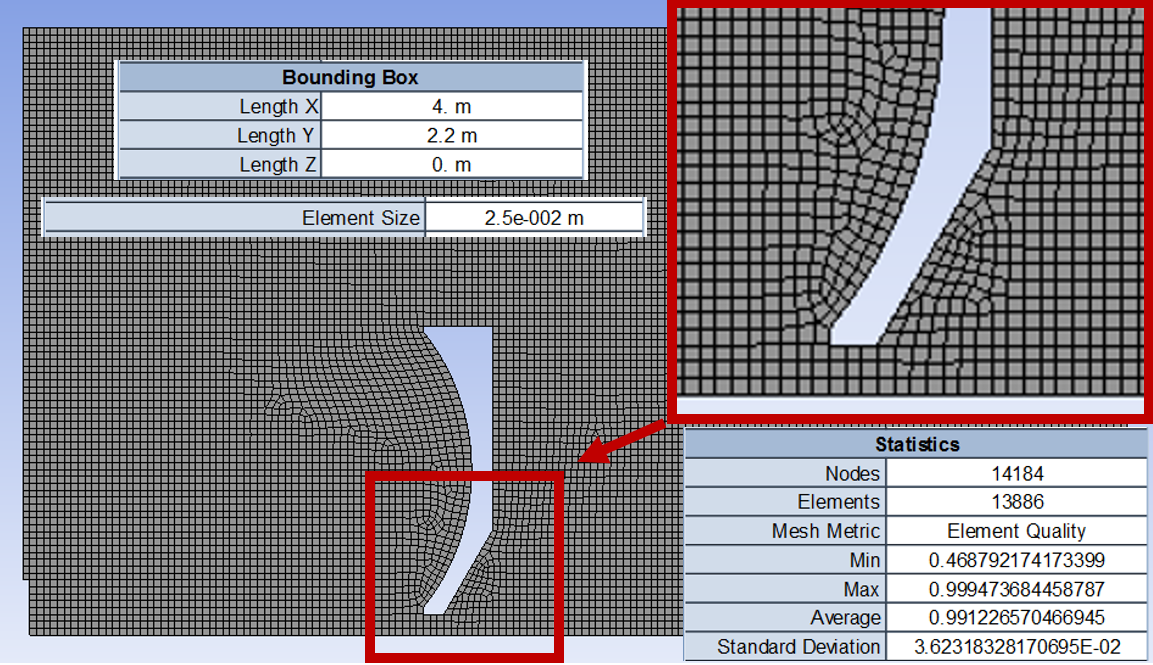
\includegraphics[width=\linewidth]{figures/cfd_mesh.png}
    \caption{Example of a discretized mesh of finite elements used for a CFD fluid flow simulation.}
    \label{fig:cfd_mesh}
\end{figure}

After deciding the scale which we are interested in modeling and studying, the next step is to define the relevant geometry, fluids, and boundary conditions for the simulation as show in Figures \ref{fig:cfd_geometry} and \ref{fig:cfd_boundary_conditions} below. Lastly, a solver is selected and the simulation is run for a specific period of time.

\begin{figure}[H] \centering
    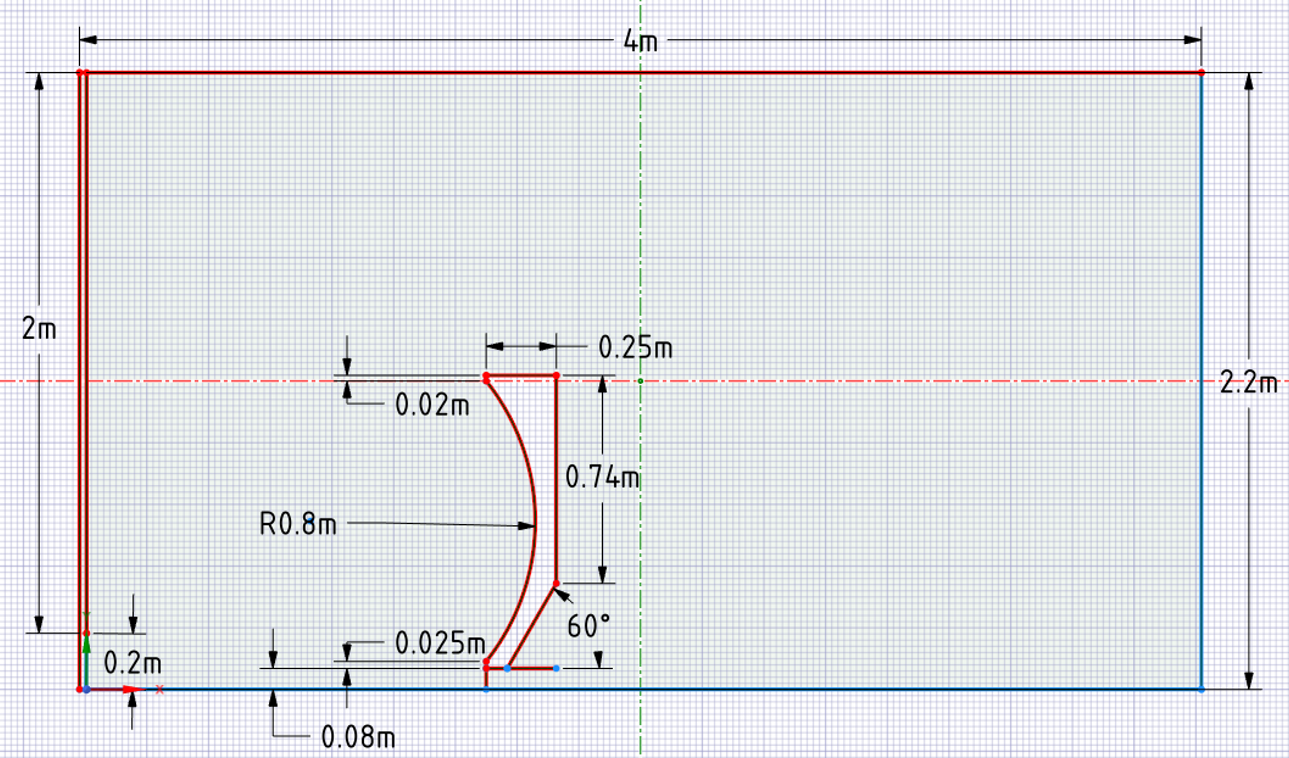
\includegraphics[width=\linewidth]{figures/cfd_geometry.png}
    \caption{Example of geometry used for a CFD fluid flow simulation. This modeled geometry is for a proposed water-braking mechanism for a pusher sled system used in the Holloman Air Force Base for experiments.}
    \label{fig:cfd_geometry}
\end{figure}

\begin{figure}[H] \centering
    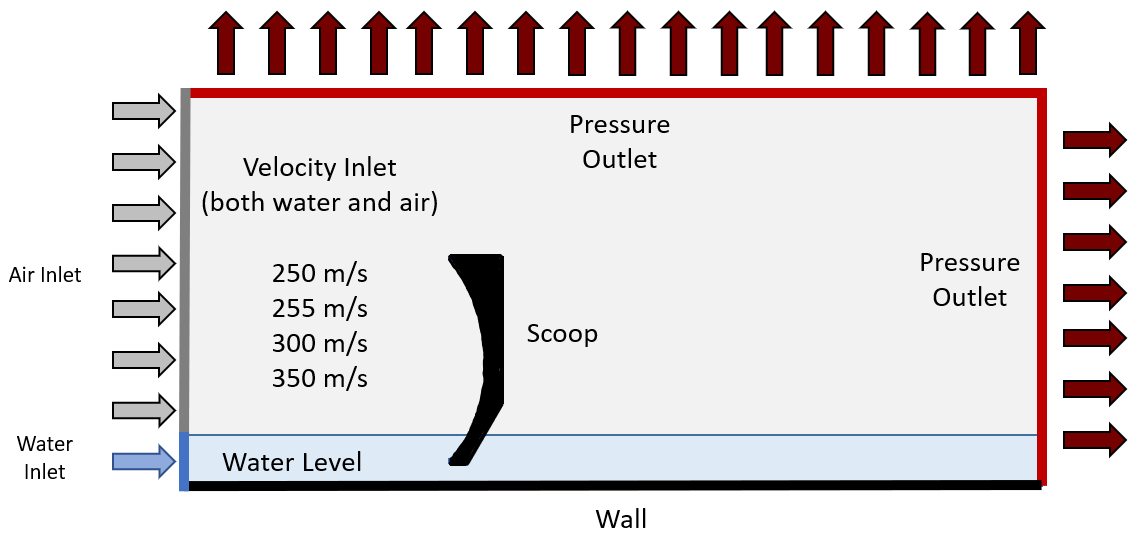
\includegraphics[width=\linewidth]{figures/cfd_boundary_conditions.png}
    \caption{Example of boundary conditions used for a CFD fluid flow simulation. These boundary conditions model how the geometry (water-breaking scoop) will interact with the water as the pusher sled mechanism pushes the scoop at specific initial velocities.}
    \label{fig:cfd_boundary_conditions}
\end{figure}

One drawback of CFD simulations is that high-fidelity simulations can be very computationally expensive as having smaller finite elements, bigger meshes, bigger geometries, and bigger simulation environments increases the computations needed for the solvers to simulate each given time-step of the simulation. Although fluid flow datasets are available for some problems in fluid dynamics, many researchers are interested in fluid flows for specific problems with different geometries and boundary conditions than those in the available datasets. As fluid flows are a widely studied area in mechanical engineering in the field of fluid dynamics, we know that the Navier-Stokes equations can be used to describe some of these flows and that these equations are partial differential equations (PDEs) allowing us to leverage Physics-Informed Neural Networks \cite{PINNS} to tackle this limited data problem.

\subsection{Glacial Ice Segmentation}
Glaciers are a very important source of water for people and wildlife of many different regions of the world, as not only do they provide a source of drinking water but also water for watering crops and generating hydroelectric power \cite{GlacierImportance}. As these regions rely heavily on glacial melt as a water source, it is important to monitor and keep track of changes that happen to these glaciers over time. 

There exists multiple satellites such as NASA's Landsat-7, Landsat-8, and Sentinel-2 that have captured hyperspectral images of these glaciers over a long period of time, allowing glaciologists to take these images and use their expertise to determine what areas of the images are clean ice, debris covered ice (ice mixed with rocks), and regular rocks in a process called glacier mapping. This is one of the ways that these scientists monitor the glaciers over time, and in the area of computer vision is called image segmentation. An example of this is given in Figure \ref{fig:glacier_mapping} below.

\begin{figure}[H] \centering
    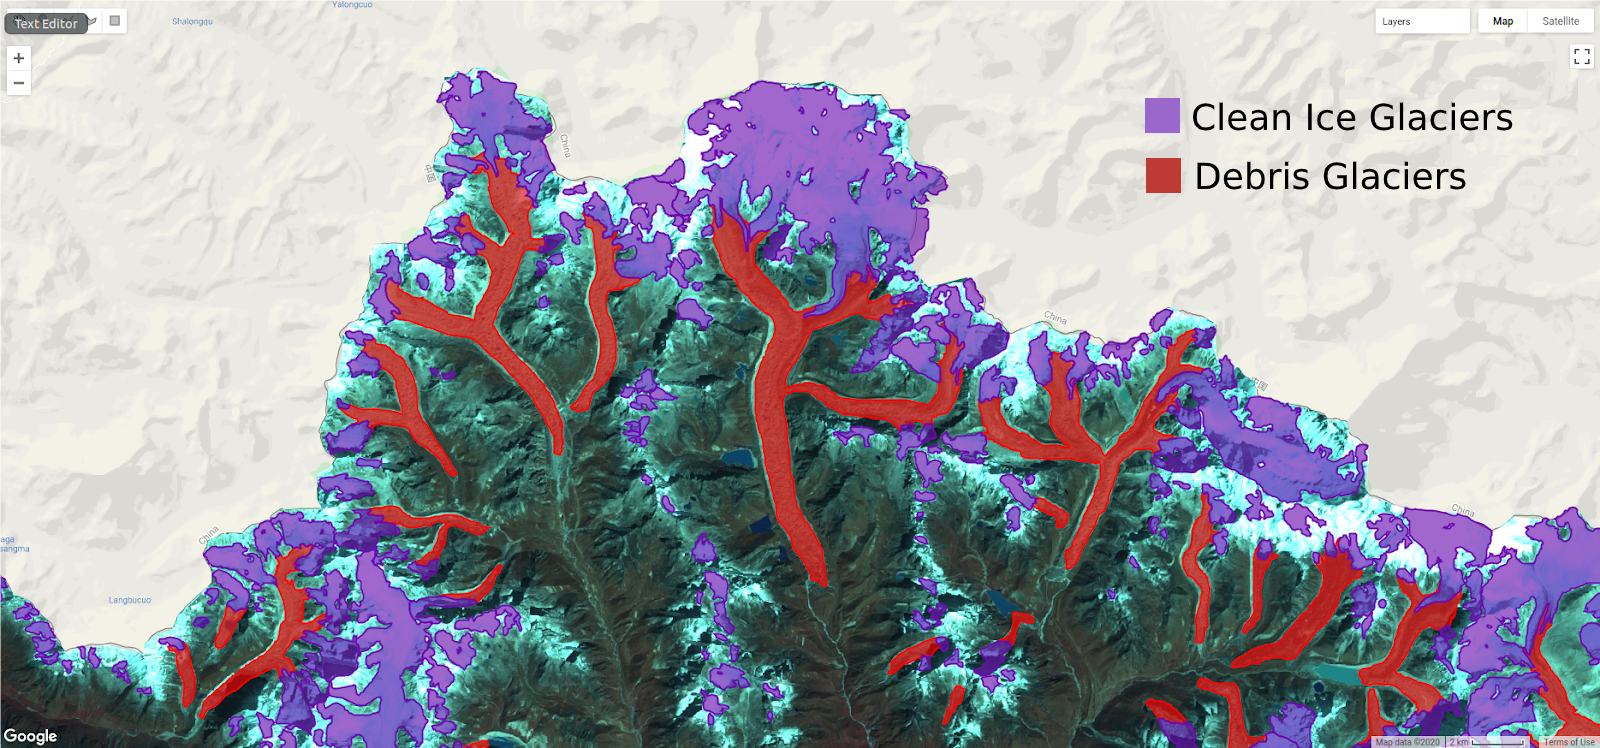
\includegraphics[width=\linewidth]{figures/glacier_mapping.png}
    \caption{Example of glacier mapping or segmentation of a satellite image into clean ice and debris covered ice glaciers.}
    \label{fig:glacier_mapping}
\end{figure}

However, manually labelling hyperspectral satellite images into clean ice and debris covered ice glaciers is a very time consuming task. This is due to two main reasons:

\begin{itemize}
    \item Satellite images have more channels than the regular 3 (RGB) in digital cameras, so they are hyperspectral images and require the usage of specialized tools (like QGIS) and knowledge about what channels capture which bands of the electromagnetic spectrum to properly visualize and analyze.
    \item High resolution images are difficult to segment as there are too many individual pixels, and although glaciologists use tools such as QGIS to label the images using geometric shapes instead of pixel by pixel to speed up the process it is still time consuming and difficult to label the borders/boundaries between the clean ice and debris covered ice specifically due to the amount of fine detail and care needed.
\end{itemize}

Labeling a single patch of a glacier using Sentinel-2 satellite imagery can take an expert 1 to 4 weeks depending on the complexity of the image, and the Hindu-Kush Himalayas (HKH) glaciers are made up of at least 256 of such patches.

A labeled dataset exists for the glaciers in Hindu-Kush Himalayas (HKH) region created by the International Centre for Integrated Mountain Development (ICIMOD) for images taken with NASA's Landsat-7 satellite. These images contain 7 channels including RGB, Near-Infrared, and Digital Elevation Map data. 

There also exists a dataset of glacier ice velocities created by the National Snow and Ice Data Center containing the surface velocities of major glacier-covered regions in the world including the Hindu-Kush Himalayas (HKH) spanning from 1985 to 2018 and compiled from multiple of NASA's Landsat satellites called the ``MEaSUREs ITS\_LIVE Regional Glacier and Ice Sheet Surface Velocities'' dataset. As glacial ice velocity prediction is a specialized form of fluid velocity prediction where the fluid being analyzed is ice from the glaciers, we can use the Navier-Stokes equations once again to leverage Physics-Informed Neural Networks \cite{PINNS} to help us tackle this limited data problem.

\section{Thesis Statement}
% Using partial differential equations
% physics-informed data augmentation and loss function design
% a little more specific towards the work I completed
Incorporating physics in neural network models through modification of data and loss functions will allow for better performance and faster convergence for the problems of fluid flow velocity prediction and glacial ice segmentation.

% \begin{enumerate}
%     \item \textbf{Problem Determination} - Determining what exactly is the problem we want to solve and how to set it up as a data problem that can be solved using machine learning (ML) models. 
%     \item \textbf{Data Gathering} - Collecting or finding a source of data for the problem we want to solve.
%     \item \textbf{Baseline Preparation} - Determining and implementing baselines to determine if our approach is actually doing better than other approaches and what metrics should be used for comparison and evaluation.
%     \item \textbf{Neural Network Architecting} - Determining what neural network architecture will be used and what other techniques from few-shot learning need to be applied to solve this problem.
%     \item \textbf{Experimentation} - Training and evaluating different neural networks to find the best performing model.
% \end{enumerate}

% I defined the fluid flow velocity prediction problem as the ML task called ``Next-Frame Prediction'' and the glacial ice segmentation problem as the ML task called ``Image Segmentation''. In each chapter I will be discussing approaches I used or propose to use to solve these tasks in detail along with the specific data gathered, baseline preparations, network architectures, and experimental results. The bulk of my research contributions will be in the architecting of the neural networks as that is where I will be integrating the physics into the models. I will specifically do so by creating new loss functions, new architectures based on previously proposed literature models, and by augmenting the limited data I gathered with ``Physics-Aware'' input channels.

\section{Expected Contributions}
The proposed contributions of this research are as follows:

% **SPLIT FURTHER... GENERALIZE NO NEED FOR SPECIFICS.. VARIABLES MISSING (TEMPERATURE, ETC) BUT WE KNOW VERY LITTLE IN GLACIER MAPPING VS FLUID FLOW. INVESTIGATE NETWORKS THAT EXPLOIT SEQUENCE...ETC..WAYS TO AUGMENT DATA...**

% A lot of variables => Be specific
% Typically, all scales/times discretized like in the fininte element method
% My idea is to exploit the fact that the laws of physics have to be followed / the real world follows the laws of physics / there are some things that the neural network does not need to learn
% 

\begin{enumerate}
    \item \textbf{A physics-informed neural network model for the task of fluid flow velocity prediction} - We will develop a model that uses Physics-Informed Neural Networks (PINNs) \cite{PINNS} for the task of fluid flow velocity prediction and investigate ways to combine PINNs with networks built for sequential data (such as \cite{LSTM}) to take advantage of how fluid flows over time sequentially allowing for improvements on network convergence speed.

    \item \textbf{A neural network model with physics-informed data augmentation for the task of glacier mapping} - As there already exists a network for glacier mapping by image segmentation \cite{Bibek2023}, we will investigate ways to augment the current available labeled data for glacier mapping based on physics, improving the performance of the pre-existing segmentation model. 

    \item \textbf{A physics-informed neural network model for the task of glacial ice velocity predictions} - Glacial ice velocity prediction is a subset of the general fluid flow velocity prediction problem, allowing us to use Physics-Informed Neural Networks (PINNs) \cite{PINNS} combined with networks built for sequential data (such as \cite{LSTM} and \cite{Attention1}) to leverage the fact that glacial ice flows over time (sequentially) for the task of glacial ice velocity prediction.

    \item \textbf{A physics-informed neural network model for the task of glacier mapping} - We will develop a new model based on a combination of Physics-Informed Neural Networks (PINNs) \cite{PINNS} and a pre-existing segmentation model \cite{Bibek2023} for the task of glacier mapping by segmenting glacier ice in satellite images. We will investigate ways to combine datasets containing hyperspectral satellite images that have no velocity information and datasets of ice glacier velocities to leverage the knowledge we have about the physics of ice glacier velocity flows and achieve better performance on the segmentation of glacier ice.

    % \item \textbf{A neural network architecture with physics-informed data augmentation for the task of glacier mapping} - There are a lot of variables that affect how glaciers behave in the real world and although we can observe them with satellites and sensors the current datasets for glacier mapping do not always include these variables at every point in time and at every scale. As there already exists a network for glacier mapping by image segmentation \cite{Bibek2023}, we will investigate ways to augment the current available labeled data for glacier mapping based on physics, improving the performance of the pre-existing segmentation model. 
    
    % \item \textbf{A physics-informed neural network architecture for the task of glacial ice velocity predictions} - Glacial ice velocity prediction is a subset of the general fluid flow velocity prediction problem so we know there are a lot of variables affecting it that are not present in the current labeled datasets. We will develop a model that uses Physics-Informed Neural Networks (PINNs) \cite{PINNS} to capture and model some of those intrinsic variables and investigate ways to combine PINNs with networks built for sequential data (such as \cite{LSTM} and \cite{Attention1}) to leverage the fact that glacial ice flows over time (sequentially) for maximum performance on the task of glacial ice velocity prediction.
    % \item \textbf{A physics-informed neural network architecture for the task of glacier mapping} - We will develop a new architecture based on a combination of Physics-Informed Neural Networks (PINNs) \cite{PINNS} and a pre-existing segmentation model \cite{Bibek2023} for the task of glacier mapping by segmenting glacier ice in satellite images. We will investigate ways to combine datasets containing hyperspectral satellite images that have no velocity information and datasets of ice glacier velocities to leverage the knowledge we have about the physics of ice glacier velocity flows and achieve better performance on the segmentation of glacier ice.
    
    
    % \item \textbf{A neural network architecture for time series data that incorporates physics for the task of fluid flow velocity predictions} - We developed Physics-Informed LSTMs \cite{Perez2022}, a novel architecture combining Physics-Informed Networks (PINNs) \cite{PINNS} and Long Short-Term Memory Networks (LSTMs) \cite{LSTM}, and tested them with fluid flow simulation data, demonstrating the viability of using physics to improve performance in terms of training speed and accuracy on neural networks with limited data. We will apply this architecture to glacier velocity data and experiment with different modifications to the architecture to find an optimal architecture for the glacier mapping task.
    % \item \textbf{A neural network architecture for hyperspectral satellite images that incorporates physics for the task of glacier mapping} - We developed Physics-Informed Data Augmented UNet, a model which computes an extra channel from the hyperspectral satellite images based on some assumptions made through observation of glacier physics, and through it demonstrated the viability of using physics to improve performance on the task of glacier segmentation. We will develop a novel architecture that combines Physics-Informed Neural Networks (PINNs) \cite{PINNS} and UNet \cite{UNet} which will be able to be used for that same task.
    % \item \textbf{Tool for faster glacier mapping} - We will develop a semi-automated system for the mapping of glaciers given hyperspectral satellite images. This system will use the models trained for glacier ice segmentation that are augmented with physics proposed in \#2 and produce masks of glacier labels that can then be loaded in QGIS, a tool often used by glaciologists for manual glacier mapping. Glaciologists will then be able to edit and correct these masks, speeding up the manual mapping process as they won't have to start from scratch for every single image they want to label.
\end{enumerate}

% \newpage
% \section{Timeline}
% To view the current graphical timeline more clearly, please see it on Google Docs:
% \url{https://docs.google.com/spreadsheets/d/1QdJVmF3Ofcg3Fgk2A4Auc5od6M4ocpm2C0jPb-eUnIQ/edit?usp=sharing}

% \begin{figure}[hbtp]
%     \makebox[\linewidth]{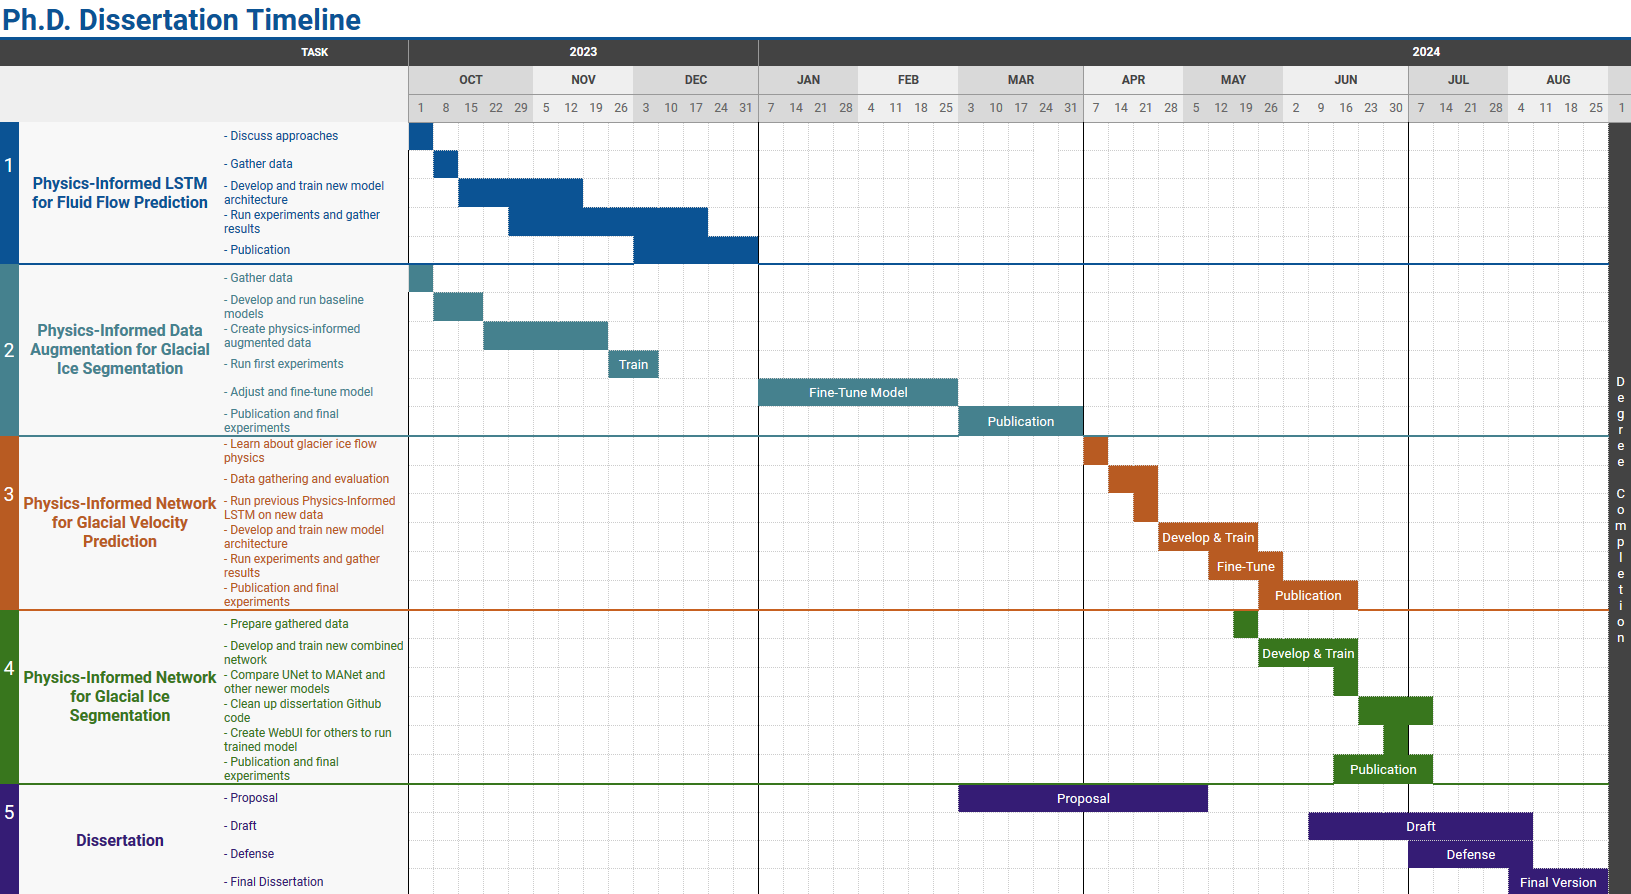
\includegraphics[scale=0.5]{phd_timeline.png}}
%     \caption{Proposed timeline visualized graphically.}
%     \label{fig:timeline}
% \end{figure}

% The table below breaks down the timeline per task, and many tasks will be running concurrently throughout the timeline.
% \begin{table}[ht!]
%     \centering
%     \begin{tabular}{l|c}
%         \toprule
%          Task & Duration \\ 
%          \midrule
%          \textbf{Physics-Informed LSTM for Fluid Flow} & 3 Months \\ \hline
%          - Discuss approaches with Dr. Kumar's students & 1 Week \\
%          - Gather data from Dr. Kumar's students & 1 Week \\
%          - Develop and train new model architecture & 5 Weeks \\
%          - Run experiments and gather results & 8 Weeks \\
%          - Publication & 5 Weeks \\ \hline
%          \textbf{Physics-Informed Data Augmentation for Glacial Ice Segmentation} & 3 Months \\ \hline
%          - Data gathering & 1 Week \\
%          - Baseline models & 2 Weeks \\
%          - Created physics-informed augmented data & 5 Weeks \\
%          - First experiments & 2 Weeks \\
%          - Adjustments to model and data for improved performance & 8 Weeks\\
%          - Publication & 5 Weeks \\ \hline
%          \textbf{Physics-Informed Net for Glacial Velocity} & 3 Months \\ \hline
%          - Learning about glacier ice flow physics & 1 Week \\
%          - Data gathering and evaluation & 1 Week \\
%          - Running previous Physics-Informed LSTM on new data & 1 Week \\
%          - Creating and evaluating new architecture & 1 Month \\
%          - Running final experiments & 1 Week \\
%          - Publication & 3 Weeks \\ \hline
%          \textbf{Physics-Informed Net for Glacial Ice Segmentation} & 3 Months \\ \hline
%          - Gathering data for the combined network & 1 Week \\
%          - Training and evaluating methodology 1 for combining networks & 2 Weeks \\
%          - Training and evaluating methodology 2 for combining networks & 2 Weeks \\
%          - Comparing UNet to MANet and other newer models & 1 Week \\
%          - Cleaning up all dissertation Github code for other researchers to use & 2 Weeks \\
%          - Creating simple WebUI tool for glaciologists to use our trained models & 1 Week \\
%          - Publication & 3 Weeks \\ \hline
%          \textbf{Dissertation} & Dates \\ \hline
%          - Defense & 07/24 - 08/24 \\
%          - Final dissertation submitted & 08/24 - 09/24 \\
%          \bottomrule
%     \end{tabular}
%     \caption{Proposed timeline to complete all dissertation tasks.}
%     \label{tab:timeline}
% \end{table}
\include{chapter2_related_works}
\chapter{Physics-Informed LSTM Network For Velocity Prediction of Fluid Flow Simulations}
\section{The Importance of Fluid Flow Velocity Prediction}
In fluid flow velocity prediction you model a system that describes some physical geometry and specific fluids with some initial boundary conditions and predict how these fluids will flow and interact in the system and what the fluid velocities will be at every point in the system after a certain amount of time has passed given the initial boundary conditions. This problem is important in mechanical engineering as the mechanical designs of airplane wings, turbines, and other important machinery are based on how they will interact with the flow of air, water, and other particles in the atmosphere or environment where they are used.

\begin{figure}[H] \centering
    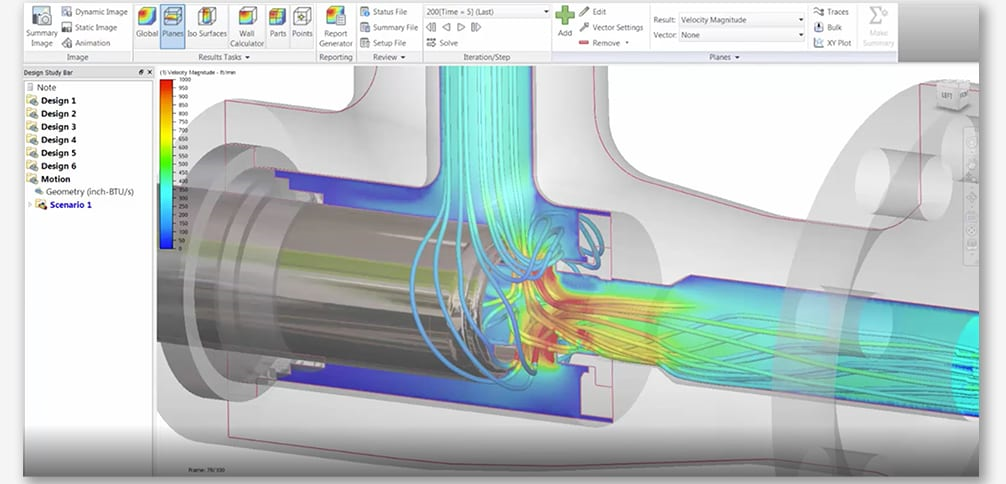
\includegraphics[width=\linewidth]{figures/cfd_engine.png}
    \caption{An example of a Computational Fluid Dynamics (CFD) simulation predicting the fluid flow velocities in an engine.}
    \label{fig:cfd_engine}
\end{figure}


\section{Long Short-Term Memory Networks (LSTMs) For Time Series Data}
\begin{figure}[H] \centering
    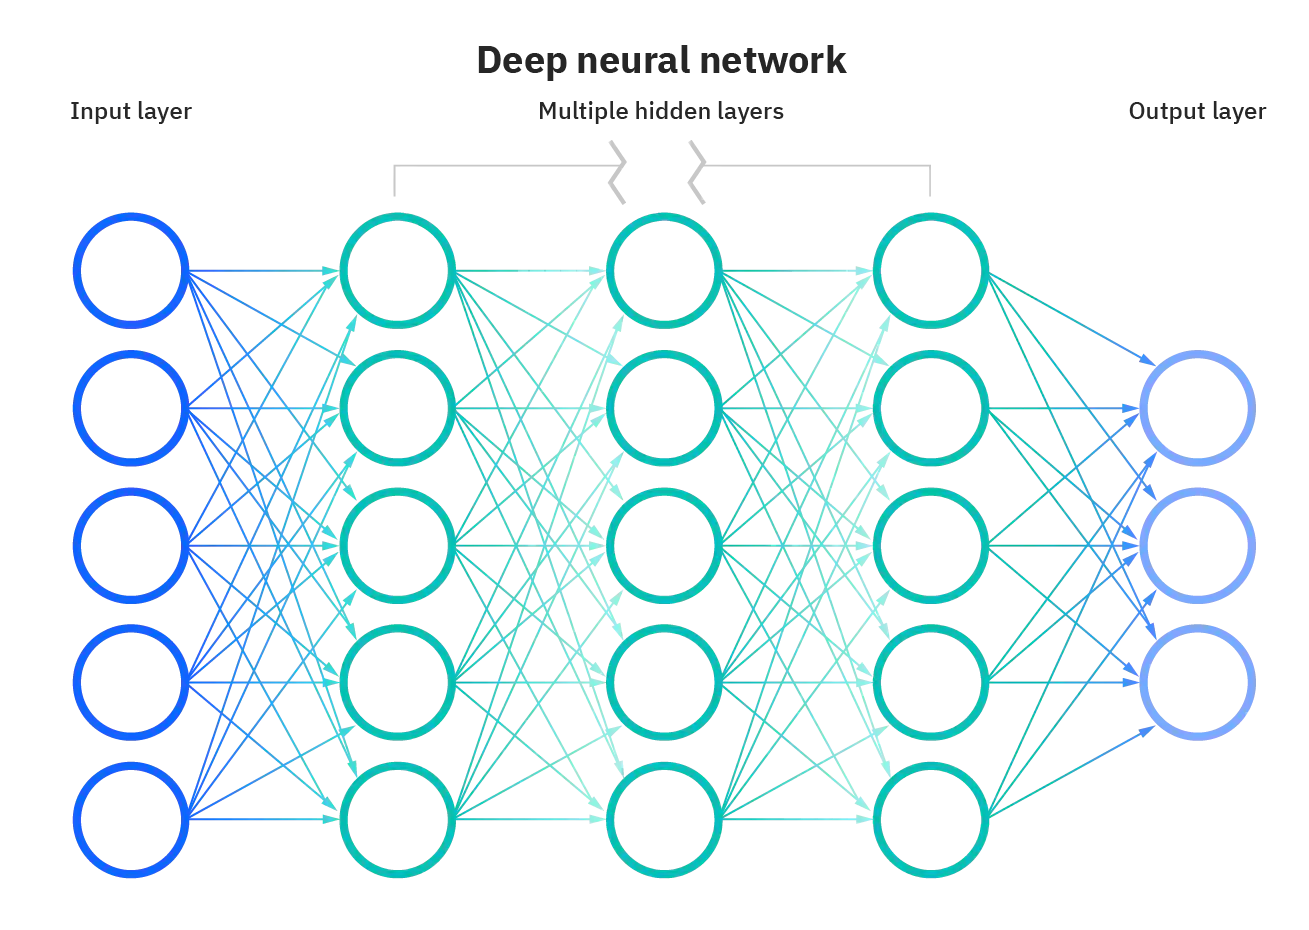
\includegraphics[width=0.4\linewidth]{figures/neural_network.png}
    \rulesep
    % https://www.asimovinstitute.org/neural-network-zoo/
    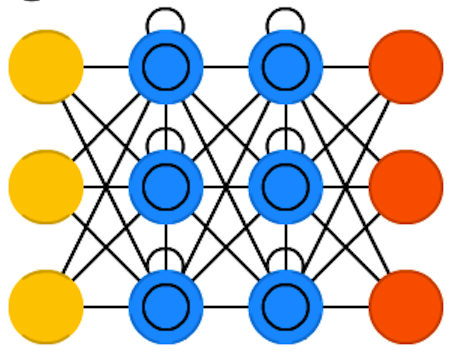
\includegraphics[width=0.4\linewidth]{figures/lstm.png}
    \caption{A regular 3-layer dense neural network on the left, an LSTM on the right. On the LSTM the blue dots with circles are the specialized LSTM cells, and note how self-connections from RNNs are present in LSTMs as well.}
    \label{fig:neural_network_and_lstm}
\end{figure}

Long Short-Term Memory Networks (LSTMs) \cite{LSTM} are neural network models designed to learn long term dependencies in sequential datasets and are a variation of the Recurrent Neural Network (RNN). LSTMs selectively pick and store short-term information that might be useful to know for later using a unique cell structure that includes an input, forget, and output gate. These gates determine what past information to forget and what new information to keep track of and it is through this mechanism of storing short memories for a long period of time where ``long'' short-term memory derives the name from.

% https://towardsdatascience.com/lstm-recurrent-neural-networks-how-to-teach-a-network-to-remember-the-past-55e54c2ff22e
\begin{figure}[H] \centering
    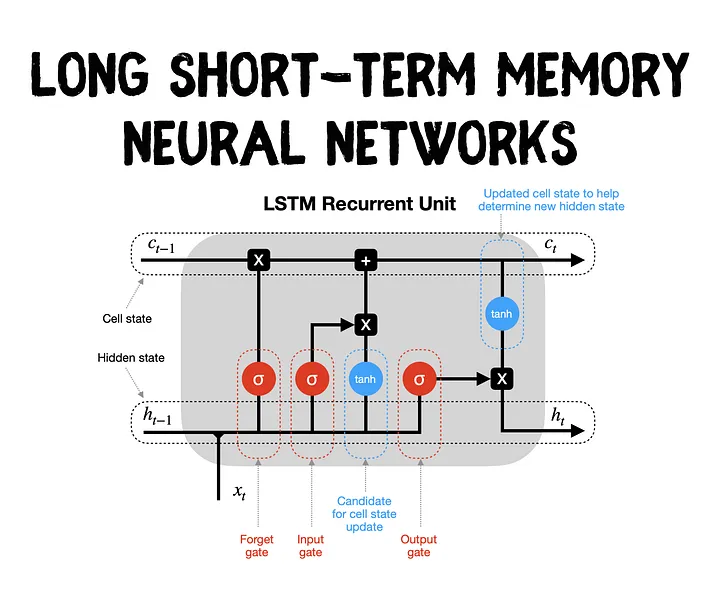
\includegraphics[width=0.8\linewidth]{figures/lstm_unit.png}
    \caption{An LSTM cell or unit showing all the gates and operations.}
    \label{fig:lstm_cell}
\end{figure}

\section{Adding Physics to LSTMs}
I began to tackle the problem of fluid flow predictions by creating a new neural network architecture based on a combination of Physics-Informed Neural Networks (PINNs) and Long-Short Term Memory Networks (LSTMs) \cite{Perez2022}. Specifically, we created a two-branch network architecture that takes as inputs the measurements taken from a Computational Fluid Dynamic (CFD) simulation and predicts what the velocity components (in 2D) will be for a given timestep.

\subsection{Fluid Flow Velocity Data From Simulations}
The data was generated using Ansys by creating a simulation in which we modeled a water-braking scoop mechanism in 2D space, constraining the domain of the model to a 2.2 meter by 4 meter box and running the simulation with different inlet velocity profiles. The simulation geometry, mesh, and boundary conditions can be seen in Figures \ref{fig:cfd_geometry}, \ref{fig:cfd_mesh}, and \ref{fig:cfd_boundary_conditions} in the Introduction section.

The following figures demonstrate the simulation results for different boundary conditions at specific times in the simulation. For the figures with two pictures, the left picture represents the pressure and velocity contours and the right picture the velocity and water volume fraction.

\begin{figure}[H] \label{fig:fluid_sim1} \centering
    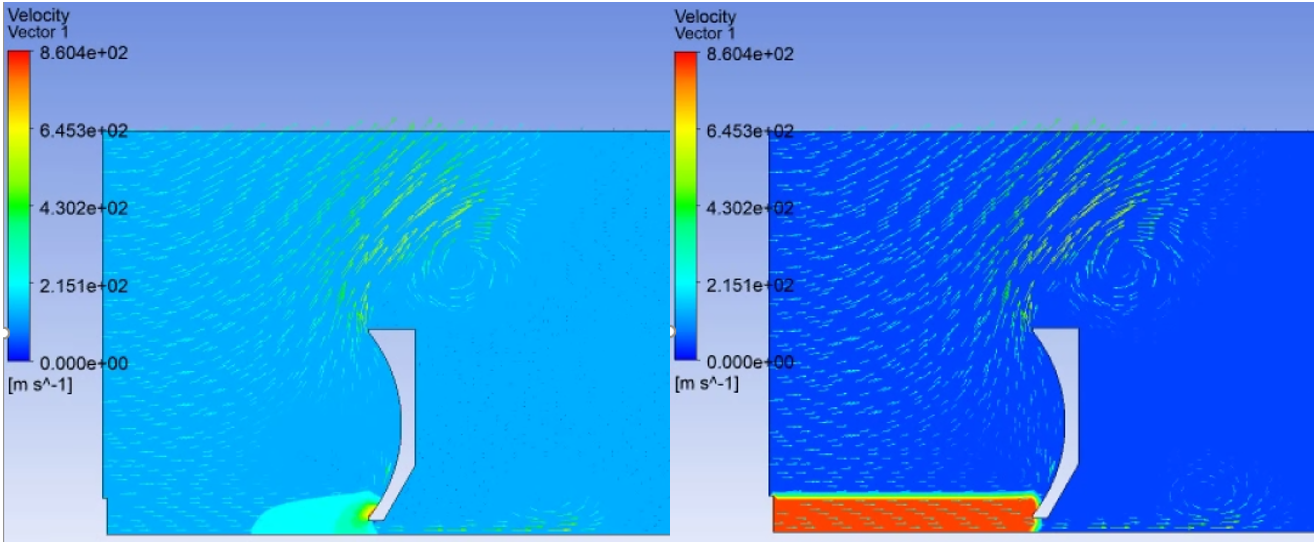
\includegraphics[width=\linewidth]{figures/fluid_sim1.png}
    \caption{Velocity Inlet = $250 m/s$, Time = $0.011sec$}
\end{figure}

\begin{figure}[H] \label{fig:fluid_sim3} \centering
    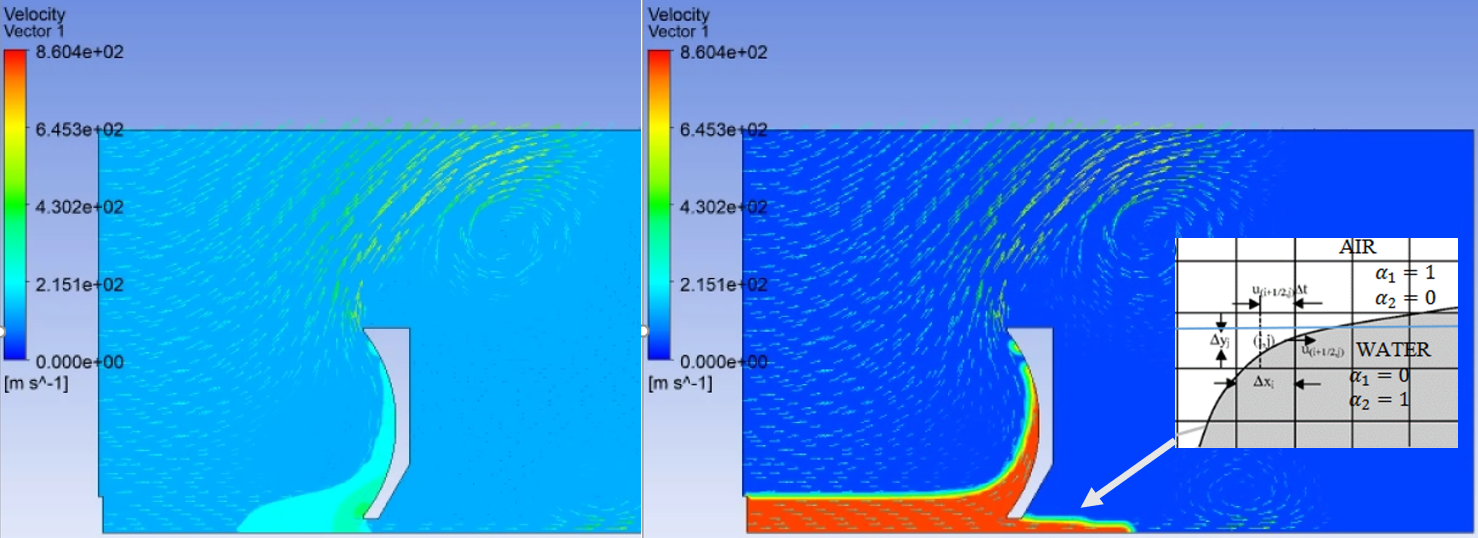
\includegraphics[width=\linewidth]{figures/fluid_sim3.png}
    \caption{Velocity Inlet = $250 m/s$, Time = $0.016sec$.}
\end{figure}

\begin{figure}[H] \label{fig:fluid_sim2} \centering
    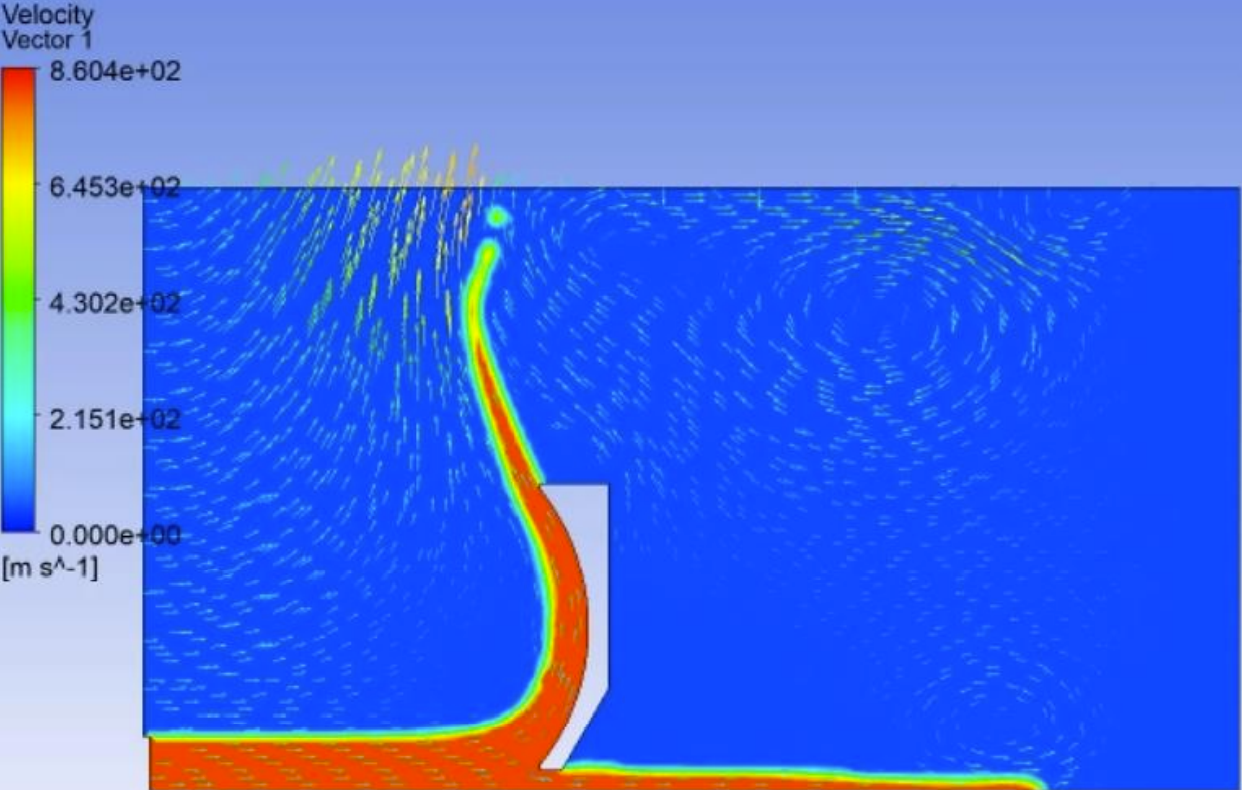
\includegraphics[width=\linewidth]{figures/fluid_sim2.png}
    \caption{Velocity Inlet = $250 m/s$, Time = $0.025sec$}
\end{figure}

The 7 measurements stored for each data sample in the simulation were:
\begin{itemize}
    \item The x-coordinate of the node, $x$
    \item The y-coordinate of the node, $y$
    \item The timestep, $t$
    \item The pressure (in atmospheres), $p$
    \item The u-velocity representing the x-component of the velocity field, $u$
    \item The v-velocity representing the y-component of the velocity field, $v$
    \item The water volume fraction or percentage of water from 0 to 1, $w.vf$
\end{itemize}

From now on, we will refer to data samples with the letter $x$, so for example $x^p$ is the pressure of the sample $x$ and $x_t^p$ is the pressure of the sample $x$ at a specific point in time $t$.

\subsection{Measuring Network Performance With The Mean Squared Error}
To measure the performance of our neural network we used a metric called \textbf{Mean Squared Error} which computes how erroneous our predictions were on average from the real values. The metric is defined in Equation \ref{eq:mse} below.
\begin{equation} \label{eq:mse}
    \frac{1}{n} \sum_{i=1}^{n}(y_{pred}-y_{true})^2
\end{equation}

where $y_{true}$ was the real value, $y_{pred}$ was our predicted value, and $n$ was the number of values or samples we were comparing.

For perfect predictions the value of $MSE = 0$. Therefore, the closer to 0 the better a model is performing.

\subsection{Proposed Network Architecture}
The proposed two-branch neural network took a range of time of measurements as input called the ``lookback'' and outputted the velocity components $u$ and $v$ that were predicted for the same position in space for the next timestep. The LSTM branch incorporated knowledge about the sequence and the Physics-Informed branch incorporated knowledge about the Partial Differential Equations (PDEs) describing in-compressible 2D discrete Navier-Stokes fluid flows. The architecture looked as follows:

% TODO: Re-render in higher quality as we have the original draw.io files
\begin{figure}[H] \label{fig:physics_lstm_architecture} \centering
    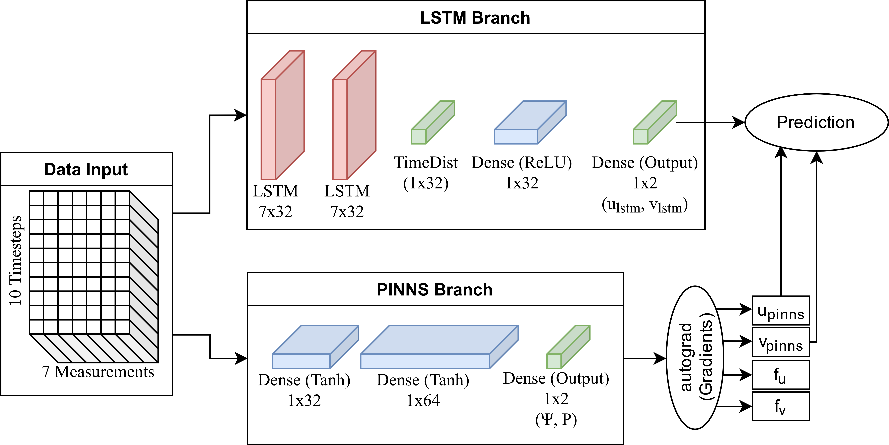
\includegraphics[width=\linewidth]{figures/physics_lstm_architecture.png}
    \caption{Physics-Informed LSTM Architecture showing both the LSTM and Physics-Informed branches and their connection to the final output prediction.}
\end{figure}

\subsubsection{LSTM Branch}
The LSTM branch had two stacked bi-directional LSTM layers with 32 activations each, followed by a Time Distributed layer that used a fully connected layer of 32 activations with a linear activation function. The Time Distributed layer applied the same weights to the previous LSTM outputs one timestep at a time. The LSTM layers were followed by a fully connected layer with 32 activations using the ReLU \cite{ReLU} non-linear activation function which was then followed by a fully connected output layer. The output layer consisted of two outputs, the x-component of the velocity field called u which was represented as $u_{lstm}$ and the y-component of the velocity field called v which was represented as $v_{lstm}$. The LSTM layers were connected to the fully connected part of the network by concatenating the two directional hidden states outputted by the last LSTM layer.

\subsubsection{Physics-Informed Branch}
As described in \cite{PINNS}, the general 2D Navier-Stokes equations:

\begin{equation} \label{eq:navier_stokes}
\begin{split}
    u_t + p_x + \lambda_1 (uu_x + vu_y) - \lambda_2 (u_{xx} + u_{yy}) &= 0 \\
    v_t + p_y + \lambda_1 (uv_x + vv_y) - \lambda_2 (v_{xx} + v_{yy}) &= 0 \\
    u_x + v_y &= 0
\end{split}
\end{equation}

We assumed that for some latent function $\psi(x, y, t)$

\begin{equation}
\begin{split}
    u &= \psi_y \\
    v &= -\psi_x
\end{split}
\end{equation}

Then we approximated $\psi(x, y, t)$ using a dense neural network $f$ with three inputs $(x, y, t)$, two outputs ($u, v$), and two learnable parameters $(\lambda_1, \lambda_2)$.

\begin{equation}
\begin{split}
    f_u(x,y,t) &:= u_t + p_x + \lambda_1 (uu_x + vu_y) - \lambda_2 (u_{xx} + u_{yy}) \\
    f_v(x,y,t) &:= v_t + p_y + \lambda_1 (uv_x + vv_y) - \lambda_2 (v_{xx} + v_{yy})
\end{split}
\end{equation}

The combined physics loss we needed to minimize was then computed from the following four losses:
\begin{equation}
\begin{split}
    MSE_u &= \frac{1}{n} \sum_{i=1}^{n}(\psi_y - u^i)^2 \\
    MSE_v &= \frac{1}{n} \sum_{i=1}^{n}(-\psi_x - v^i)^2 \\
    MSE_{f_u} &= \frac{1}{n} \sum_{i=1}^{n}(f_u(x^i,y^i,t^i))^2 \\
    MSE_{f_v} &= \frac{1}{n} \sum_{i=1}^{n}(f_v(x^i,y^i,t^i))^2
\end{split}
\end{equation}

Such that the total loss was:

\begin{equation}
    MSE_{total} = MSE_u + MSE_v + MSE_{f_u} + MSE_{f_v}
\end{equation}

The architecture consisted of a simple dense network with 3 layers. The first layer had 32 activations and used the hyperbolic tangent non-linear activation function (tanh), followed by another fully connected layer with 64 activations using tanh once again, followed by the output layer with two outputs. The automatic differentiation system included in PyTorch named \textbf{autograd} was used to compute the partial derivatives required for the computation of the final physics loss.

\subsubsection{Two-Branch Combined Model}
The two outputs of each branch were combined by using a weight $\alpha$ that was set between 0 and 1. For our experiments, $\alpha = 0.5$ (but in the future it could be set as a learnable parameter)

\begin{equation}
\begin{split}
    u_{pred} &= \alpha * u_{lstm} + (1 - \alpha) * u_{pinns} \\
    v_{pred} &= \alpha * v_{lstm} + (1 - \alpha) * v_{pinns}
\end{split}
\end{equation}

where $(u_{pred}, v_{pred})$ were the final predictions, ($u_{lstm}$, $v_{lstm}$) were the two outputs of the LSTM branch, and $(u_{pinns}, v_{pinns})$ were the two outputs of the Physics-Informed branch.


\subsection{Baseline Used To Compare Against Our Proposed Network}
The baseline used for this model was to simply assume that the velocities at the next timestep will be the same as those in the previous timestep for each data point.

\begin{equation} \label{eq:no_change_baseline}
\begin{split}
    prev_u &= x_{t}^{u} \\
    prev_v &= x_{t}^{v} \\
    y_{t+1}^{pred} &= (prev_u, prev_t)
\end{split}
\end{equation}

where $t$ was the current timestep, $x_t$ was the current data sample, $x_t^u$ was the u-velocity component of $x_t$, $y_t^v$ was the v-velocity component of $x_t$, and $y_{t+1}^{pred}$ was our predicted velocity.

\subsection{Experimental Results}
The following table summarizes the results of the experiments and provides the mean squared error for the velocity components \textbf{U} and \textbf{V} for each model along with the total training time after 200 epochs. The experiments were performed using an NVIDIA RTX 3090 and every epoch took around 27 seconds for non-informed LSTM models and 30 seconds for physics-informed LSTM models.

\begin{table}[h!] \centering
    \begin{tabular}{c|c|c|c}
        \textbf{Model} & \textbf{U} & \textbf{V} & \textbf{Time (min)} \\ \hline
        Baseline & 5.455 & 2.561 & 0.061 \\ \hline
        PINNS Only & 5709 & 12038 & 80 \\ \hline
        LSTM Only & 1.7811 & 8.6962 & 117 \\ \hline
        PINNS+LSTM & \textbf{0.4677} & \textbf{1.2794} & 142 \\ \hline
    \end{tabular}
    \caption{Comparison of the performance (MSE) of different models when using the 250m/s simulation for training and the 300m/s simulation for testing.}
    \label{tab:physics_lstm_results}
\end{table}

%LSTM ONLY TAKES 49sec for training epochs + 48 for validation except in 10_000 epoch one takes 1:28 + 1:23
% Physics-LSTM takes 1:11 + 1:03 -> 1:45 + 1:45
% PINNS takes 1:50 + 1:47

\subsection{Conclusion}
Our experimental results in Table \ref{tab:physics_lstm_results} show that the Physics-Informed LSTM outperforms the non-informed LSTM approach and leads us to our conclusion that informing the LSTM about the governing physics leads to better performance than just using LSTMs or PINNs by themselves.
\chapter{Glacial Ice Segmentation of the HKH Region With Physics-Informed Data Augmentation}
\section{The Importance of Glacial Ice Segmentation}
Glacial ice segmentation refers to the problem of gathering hyperspectral images taken by satellites of different glaciers and segmenting or delineating which areas are glacial ice, which areas are debris covered ice (ice mixed with rocks), and which areas are just rocks. This problem is important in the field of geology as monitoring the amount and location of ice from glaciers such as the ones in the Hindu Kush Himalayas (HKH) is critical as these glaciers provide a source of freshwater to a big population of the world.

\section{Image Semantic Segmentation: Grouping Similar Pixels Together}
The task of semantic segmentation refers to grouping similar or related pixels of an image together, like those of a specific object. For example, grouping all the pixels of people, roads, buildings, or trees as seen in the figure below:

% https://towardsai.net/p/l/machine-learning-7
\begin{figure}[H] \centering
    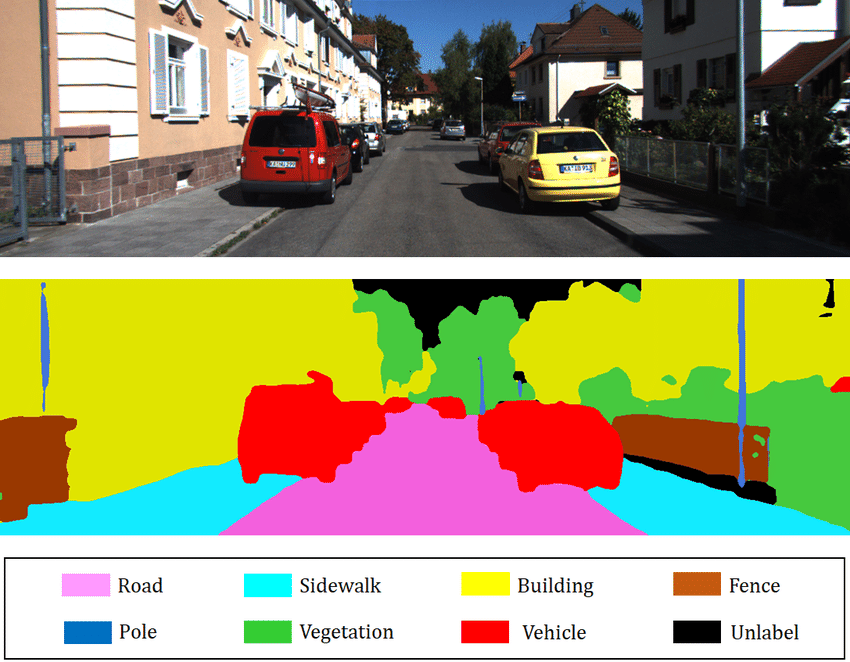
\includegraphics[width=\linewidth]{figures/semantic_segmentation.png}
    \caption{An example of semantic segmentation of an image. The pixels are grouped together by different categories.}
    \label{fig:example_semantic_segmentation}
\end{figure}

\section{Glacier Mapping Through Segmentation of Ice in Hyperspectral Images}
Glacial ice segmentation or glacier mapping is simply the task of semantic segmentation applied to hyperspectral satellite images of glaciers. The goal is to determine for each pixel in the image whether the pixel is an area of glacial ice, debris covered ice, or background (regular rocks) as shown in the figure below:

\begin{figure}[H] \centering
    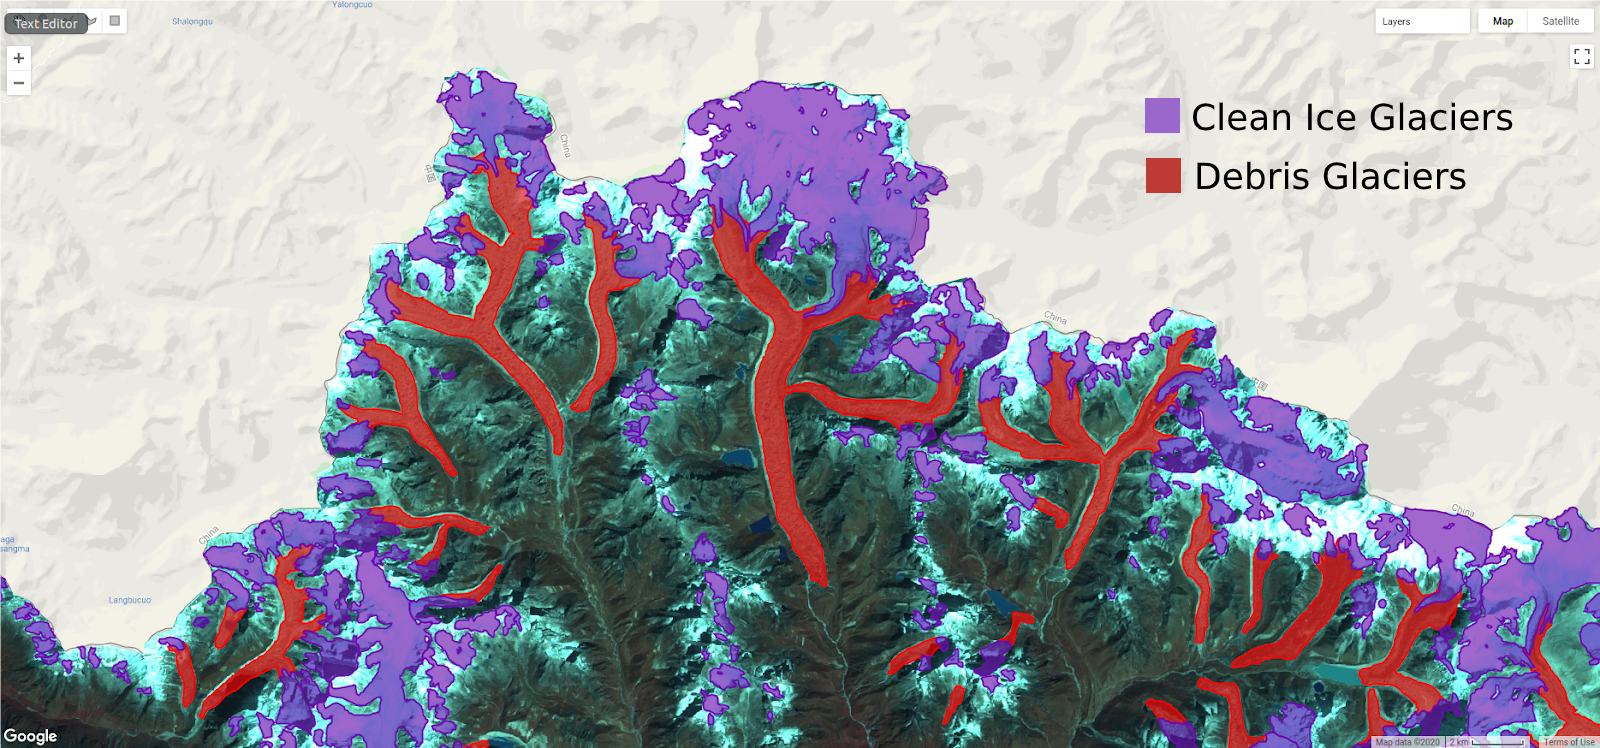
\includegraphics[width=\linewidth]{figures/glacier_mapping.png}
    \caption{Semantic segmentation of a glacier satellite image by a human annotator.}
\end{figure}


\section{Convolutional Neural Networks: The Backbone of Almost All Networks That Use Images}
Convolutional Neural Networks \cite{CNN1} are one of the most important and fundamental neural network models when dealing with datasets that contain images and their role in state-of-the-art architectures in image classification competitions such as ImageNet and other image tasks cannot be understated. CNNs operate by assuming the inputs are images and performing operations on the pixels of these images called convolutions. The purpose of these convolution operations is to apply a `filter` to extract important features out of these images as feature maps, and because these CNNs are neural networks these `filters` or `kernels` automatically learn to filter out information which might be useful for the specific task we are trying to solve. After the convolution operations a pooling operation is applied to the extracted feature maps which reduces size of these maps and the computational complexity of the network. A common pooling operation is `2x2 max-pooling` where the image is split into 2x2 patches and the maximum value at each of these patches is used to create the new reduced size feature map, the idea being that the most prominent features or those with high values are the most important for solving image problems. After extracting important features of images through convolutions and pooling layers the next step in CNNs is to convert the 2D feature maps into 1D vectors by flattening them out and then feeding these feature vectors as inputs to a regular dense network to get a final output. The layers of this dense network are typically called `fully-connected layers` to differentiate them from the `convolutional layers`.

% https://www.linkedin.com/pulse/what-convolutional-neural-network-cnn-deep-learning-nafiz-shahriar/
\begin{figure}[H] \centering
    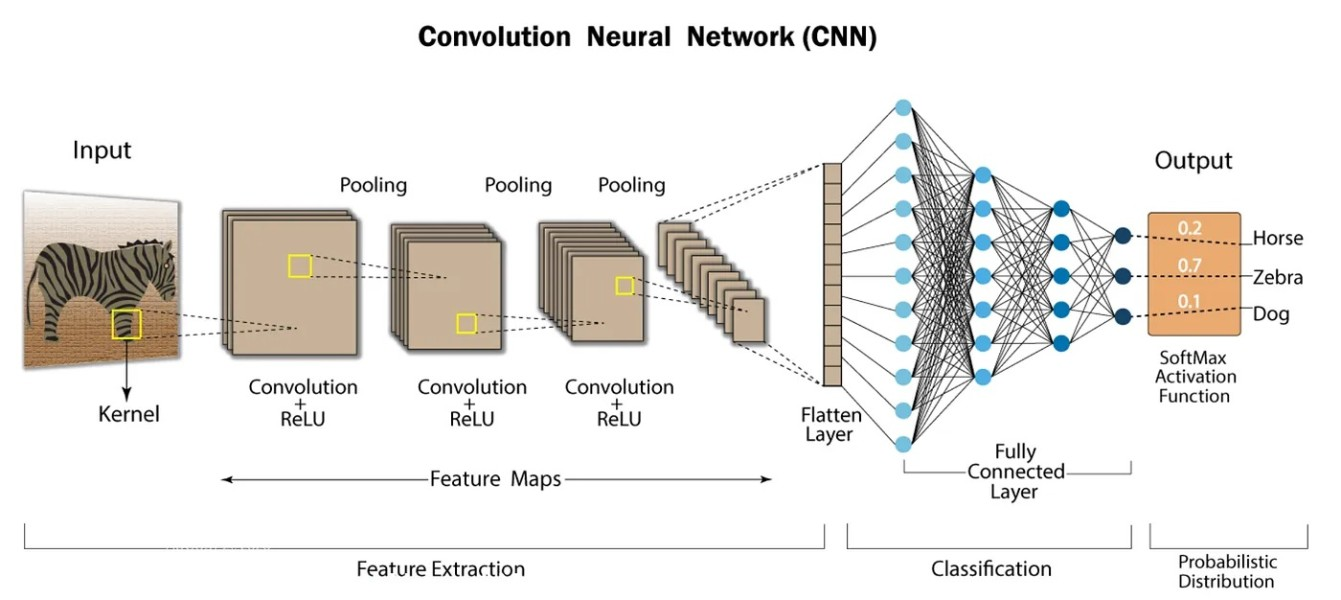
\includegraphics[width=\linewidth]{figures/cnn_architecture.jpeg}
    \caption{An example of a CNN model for an animal classification problem. Features are extracted with convolutions and pooling, and then used in a fully connected network for a final classification.}
    \label{fig:cnn_architecture}
\end{figure}


\section{UNet: The Standard Network For Image Segmentation}
U-Net \cite{UNet} is a variation of a CNN and was derived from the improvements achieved by Fully Connected Convolutional Networks (FCNs) for semantic segmentation \cite{FCN}. FCNs transform the fully-connected layers of a CNN into convolutional layers and through an upsampling strategy called `deconvolution` or `transposed convolution` output an image that is the same size as the original image. U-Net is split into two components, and encoder in the left half of the U-shape and a decoder in the right half. 

\begin{figure}[H] \centering
    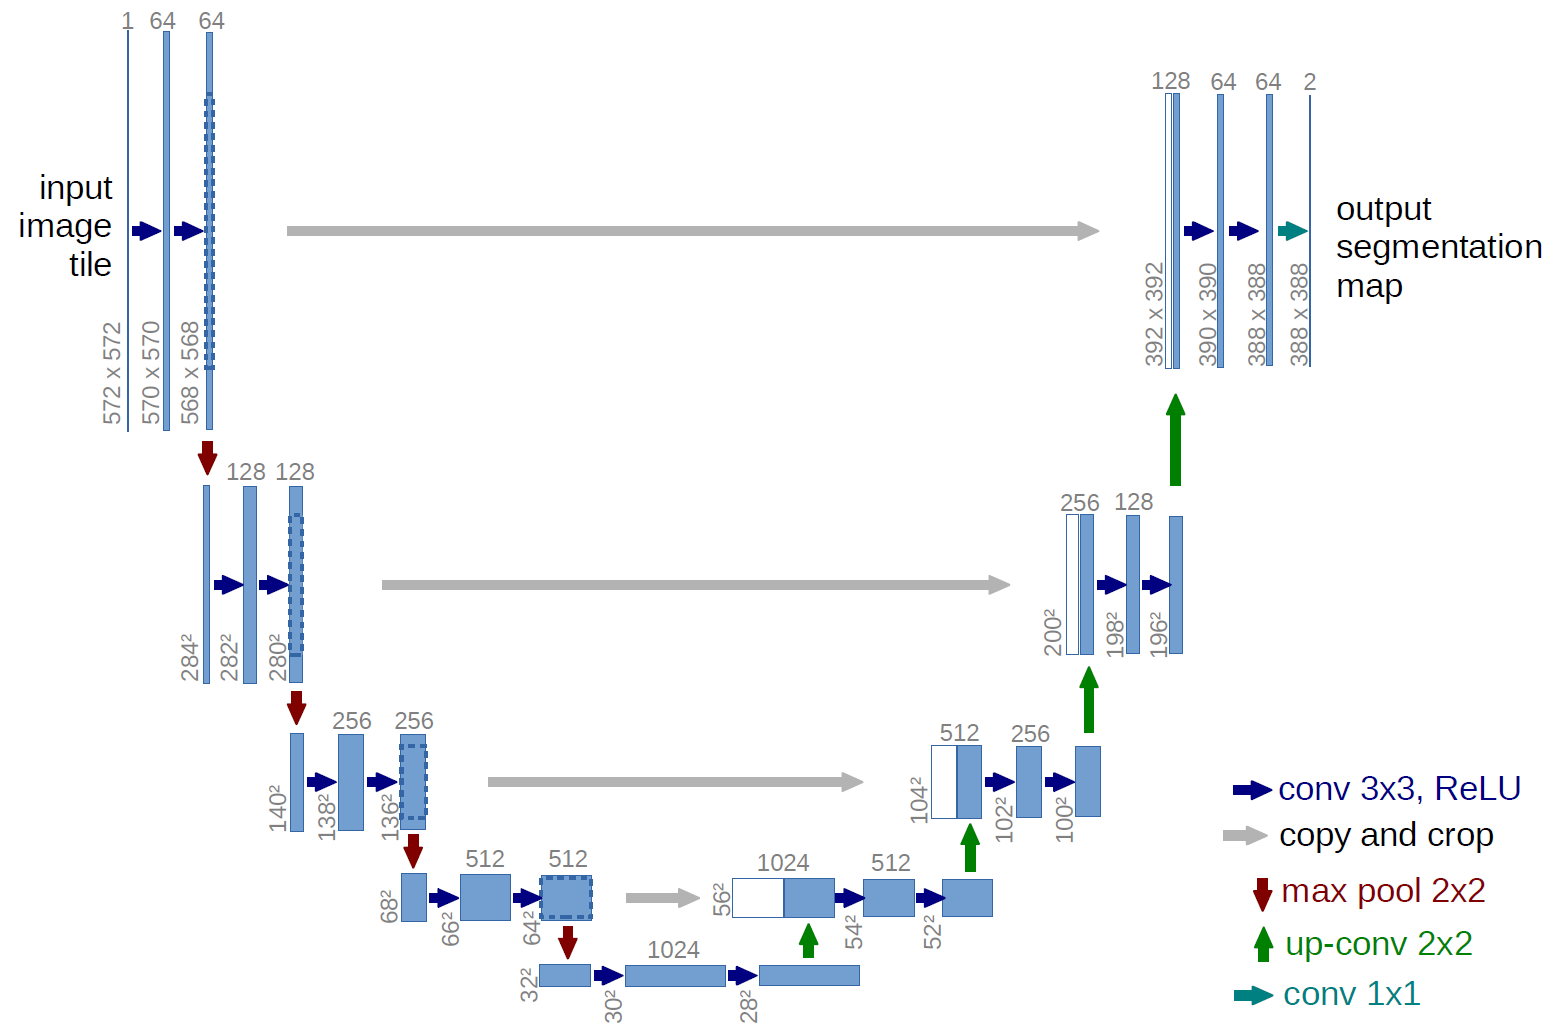
\includegraphics[width=\linewidth]{figures/unet_architecture.png}
    \caption{U-Net architecture showing both components and how they are connected to output a final segmentation map. Note the straight connections feeding previous inputs into later outputs going straight across.}
\end{figure}

The encoder also known as the contracting path is the left half of the U-shape that takes the original input image, applies regular convolutions and max-pooling, and outputs a reduced size feature map at the bottom. This is the feature extraction component that aims to capture the important context of the image.

The decoder also known as the expanding path is the right half of the U-shape that takes the feature map from the encoder and through `transposed convolutions` or `up-convolutions` upsamples and expands the feature map all the way until we get an output segmentation map which is the same size as the original input image.

Lastly, to help the decoder maintain some of the location information that is lost while encoding there are `skip-connections` going from the encoder to the decoder straight across the U-shape.

U-Net achieved state-of-the-art results when introduced in 2015 for biomedical image segmentation and these types of networks are still used to this day for many segmentation problems as a starting baseline.

\subsection{Measuring Network Performance With IoU}
% **INTRODUCING METRICS (PRECISION, RECALL, AND IOU)**
To measure the performance of the segmentation model, the main metric we used was the \textbf{Intersection over Union (IoU)} which is defined in Figure \ref{fig:iou} below and has numbers in the range from 0 to 1 with 1 being a perfect score.

\begin{figure}[H] \centering
    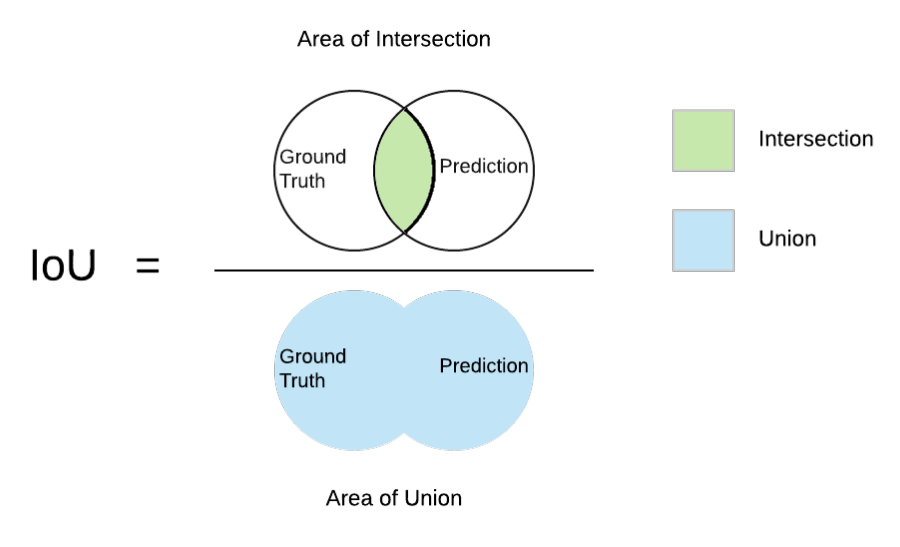
\includegraphics[width=\linewidth]{figures/iou1.png}
    \caption{Definition of Intersection over Union.}
    \label{fig:iou}
\end{figure}

\begin{figure}[H] \centering
    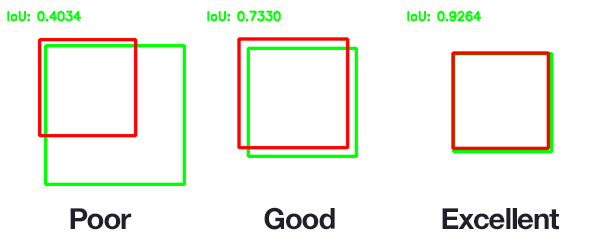
\includegraphics[width=\linewidth]{figures/iou2.png}
    \caption{Three examples of different IoU values and what type of performance they represent.}
\end{figure}

\section{Adding Physics To Image Segmentation Through Data Augmentation}
As a first step towards tackling the problem of glacial ice segmentation I began by taking a previously proposed architecture for segmentation of the Hindu Kush Himalayas (HKH) region glaciers \cite{Bibek2023} and improving its performance by adding physics to the model through data augmentation. 

The main idea was to take the elevation map from the satellite images and encode an abstract representation of a ``precipitation model'' from that elevation map as a new channel of the image. Although the actual physics equations of ice flow were not explicitly encoded in this new data channel, this new data was created from an abstract representation of the physics and we therefore called it a physics-informed data augmentation. In this channel we simulated precipitation and encoded paths where water or ice might flow from the top to the valley of the glaciers.

\begin{figure}[H] \centering
    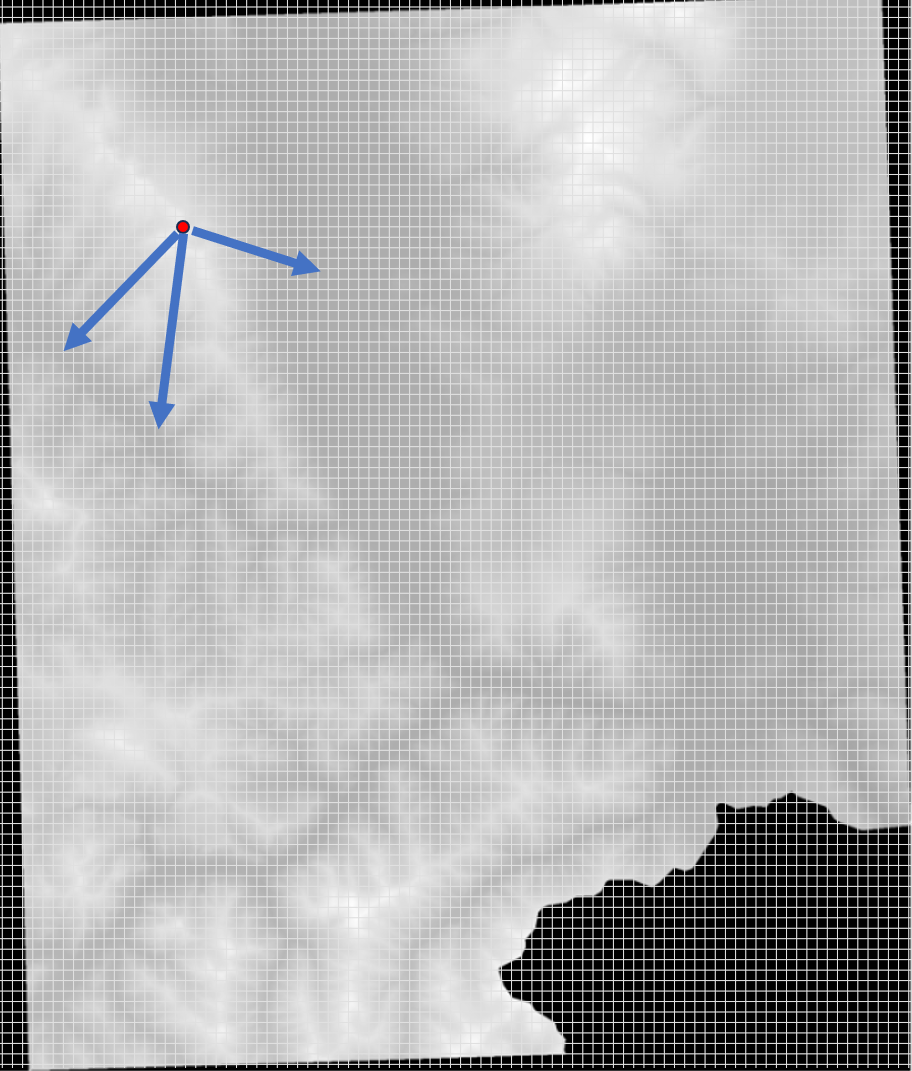
\includegraphics[width=\linewidth]{figures/data_augmentation_bfs.png}
    \caption{For each pixel in the image we simulated precipitation going down the glacier and accumulating, then we encoded such information as an additional physics-informed channel.}
    \label{fig:data_augmentation_bfs}
\end{figure}

Specifically, the algorithm as follows:
\begin{enumerate}
    \item Take the elevation map as the input image $elevation$
    \item Create an empty image of the same size as the input called $output$
    \item For each pixel in the image, perform Breadth-First Search (BFS) with a special limitation where you can only visit pixels you haven't visited before AND that are lower elevation than the current pixel popped from the queue as water/ice can only flow down.
    \item Each time a pixel is visited, the $output$ at that pixel's position increases by 1 as 1 drop of water/ice has flowed down to it.
    \item At the end, normalize the image between 0 and 1 by subtracting the mean and dividing by the standard deviation.
\end{enumerate}

In pseudocode, the data augmentation algorithm would look like:
\begin{algorithm}[H]
    \caption{Physics-Informed Data Augmentation Algorithm}
    \begin{algorithmic}
        \State $im \gets$ elevation map from satellite image
        \State $output \gets $ image full of zeros the same size as $im$
        \State $im.shape[0] \gets$ number of rows in $im$
        \State $im.shape[1] \gets$ number of columns in $im$
        \For{$u:=0 \to im.shape[0]$}
            \For{$v:=0 \to im.shape[1]$}
                \State Breadth\_First\_Search(im, output, u, v)
            \EndFor
        \EndFor
        \State $im = (im - im.mean()) / im.std()$
    \end{algorithmic}
\end{algorithm}

With the modified BFS algorithm being:
\begin{algorithm}[H]
    \caption{Physics-Informed Breadth-First Search}
    \begin{algorithmic}
        \State $im \gets$ elevation map from satellite image
        \State $output \gets$ previous accumulated output from other pixels
        \State $u \gets$ row of source pixel
        \State $v \gets$ column of source pixel
        \State $source \gets (u, v)$

        \State $visited = {source}$
        \State $Q = $ Queue with $source$ appended to it

        \While{$Q \neq Empty$}
            \State $x = Q.pop()$
            \State $curr\_elevation \gets im[x]$

            \If{$x \neq source$}
                \State $output[x] += 1$
            \EndIf

            \For{$n$ in $get\_neighbors(im, x)$}
                \State $n\_elevation \gets im[n]$
                \If{$n$ not visited $\And n\_elevation < curr\_elevation$}
                    \State Add $n$ to $visited$
                    \State Append $n$ to $Q$
                \EndIf
            \EndFor
        \EndWhile
    \end{algorithmic}
\end{algorithm}

The following figure presents an example of the results after performing the augmentation.
\begin{figure}[H] \centering
    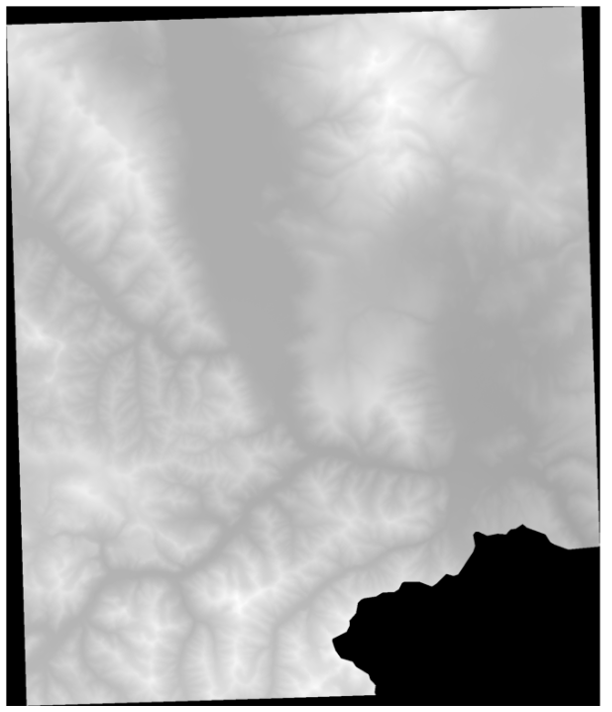
\includegraphics[width=0.45\linewidth]{figures/data_augmentation_dem.png}
    \rulesep
    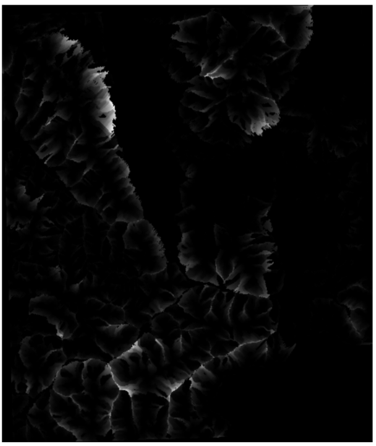
\includegraphics[width=0.45\linewidth]{figures/data_augmentation_result.png}
    \caption{Left is the elevation map from one of the glacier satellite images where white pixels are peaks and darker pixels are valleys. Right is the resulting physics-informed data augmentation channel.}
    \label{fig:data_augmentation_result}
\end{figure}


\subsection{Glacier Mapping Data From ICIMOD And Landsat7 Satellite}
The data used to train and evaluate the models were gathered and labelled by experts at the International Centre for Integrated Mountain Development (ICIMOD) from multispectral imagery from NASA's Landsat 7 satellite for the glaciers of the Hindu Kush Himalayas region from 2002 to 2008. 

\subsection{Baseline Network}
The baseline model used to evaluate our proposed data augmentation technique was the Boundary-Aware U-Net for Glacier Segmentation model developed and published in 2023 by Bibek et. al \cite{Bibek2023}. No modifications to the model were made apart from slight changes to the hyperparameter configuration and the addition of the physics-informed data augmentation technique.

\subsection{Experimental Results}
% TODO: EXPERIMENTS STILL RUNNING

% TODO: ADD IMAGE RESULTS

\begin{table}[h!]
    \centering
    \begin{tabular}{c|c|c|c}
        Model & Background IoU & CleanIce IoU & DebrisIce IoU \\ \hline
        Regular U-Net & N/A & N/A & 0.2850 \\ \hline
        Regular U-Net & N/A & 0.6560 & N/A \\ \hline
        Boundary-Aware U-Net (Baseline) & N/A & N/A & 0.3594 \\ \hline
        Boundary-Aware U-Net (Baseline) & N/A & \textbf{0.6817} & N/A \\ \hline
        \textbf{Physics \& Boundary-Aware U-Net (mine)} & 0.8640 & 0.6350 & \textbf{0.3850} \\ \hline
        
    \end{tabular}
    \caption{Comparison of the performance of different neural network models by the Intersection Over the Union (IoU) between the predicted labels and the true labels for each class. IoU is a metric between 0 and 1, with 1 being a perfect score.}
    \label{tab:my_label}
\end{table}

\subsection{Conclusion}
The current experimental results demonstrate that my proposed physics-informed data augmentation leads to improved performance for the segmentation of Debris-covered Ice from the baseline model. This is significant as classification of Debris-covered Ice is a more challenging task than that of Clean Ice for both the baseline model and expert glaciologists. With some hyper-parameter tuning I hypothesize that we can reach up to 0.40 IoU, and by switching U-Net to a newer state-of-the-art segmentation model such as MANet \cite{MANet} along with using newer loss functions such as the Unified Focal Loss \cite{UnifiedLoss} I believe we might be able to reach above 0.50 IoU. Although my proposed approach does not outperform the baseline for Clean Ice segmentation, I believe this is due to the fact that the original baseline uses two separate binary models for segmentation of each class instead of one unified multi-class model. I will train two separate binary models for a more fair comparison in the final version of my full dissertation.
\chapter{Physics-Informed Network For Glacial Ice Velocity Predictions}
As my next step, I propose making a new Physics-Informed architecture based on what I learned from the Physics-Informed LSTM Network \cite{Perez2022} which I previously applied to fluid flow simulations and adapting it to the problem of glacial ice velocity prediction. Glacial ice velocity prediction is simply the problem of fluid flow velocity prediction where the fluid is ice from a glacier. The aim of this step is to prepare a network architecture and dataset than can be later incorporated into the glacier segmentation problem as I hypothesize that including velocity information based on the physics laws of fluid flow will improve the performance of the glacier segmentation models proposed by \cite{Bibek2023}. There already exists a dataset of glacier ice velocities \cite{GoLIVE1} for satellite images created by the National Snow and Ice Data Center which can be easily adapted and incorporated with my previous methodology for velocity predictions. However, since then I have learned about newer architectures that perform better than LSTMs \cite{LSTM} such as GRUs \cite{GRU} and Transformers \cite{VIT} which I would like to try as well.

The main challenge with this step is determining how to set-up the Physics-Informed part of the network as my previous work focused on air and water flows and not ice flows. The architecture will not require many changes, it is the loss function which was based on the incompressible 2D Navier-Stokes equations which might need to be modified to accommodate the new type of data.
\chapter{Physics-Informed MANet for Glacial Ice Segmentation of the HKH Region}
As my final step, I propose combining the Physics-Informed Network used for velocity prediction and the U-Net used for image segmentation to further improve the performance on the segmentation of ice in the HKH region. I will do this by trying two different methodologies. In the first methodology, I will simply create a two branch network the same way I did with the Physics-Informed + LSTM network where we just have to carefully connect the inputs and outputs of their respective branches correctly. In the second methodology, I will use a self-learning loss that will combine the losses of both networks into one and optimize them both at the same time. The self-learning combined loss will be as follows:

\begin{equation} \label{eq:1}
    L_{Combined} = \alpha * L_{UNET} + (1 - \alpha) * L_{PINNS}
\end{equation}

where $L_{Combined}$ is the new combined loss from both networks, $L_{UNET}$ is the loss of the UNet ice segmentation network and $L_{PINNS}$ is the loss of the Physics-Informed velocity prediction network. This loss is based on the self-learning boundary aware loss specified in \cite{Bibek2023}.

The main challenge will be combining the datasets for the combined network as they were not taken at the same exact time and so the satellite images used for segmentation and the velocity images are slightly different. I do not believe this will present a major problem, as I have the script used to get both datasets so I will be able to control how far apart these datasets are in real time to minimize the error introduced by this problem. I will also try a newer segmentation architecture that has been shown to be better than UNet called MANet \cite{MANet} which I hypothesize will give me the best performance in the end.

Lastly, I will develop a simple WebUI that allows glaciologists to feed their own hyperspectral satellite images to our trained models to get labeled masks of glacial ice in a format that can be loaded into QGIS to help them with their glacier mapping efforts.

%%%%%% Bibliography %%%%%%
\printbibliography

%%%%%% CV %%%%%%
% % vitae.tex (Curriculum Vitae)

\addcontentsline{toc}{chapter}{Curriculum Vitae}
\chapter*{Curriculum Vitae}

% Patrick Thor Kahl was born on July 12, 1961. The first son of Ulf Thor Gustav 
% Kahl and Carolyn Kahl, he graduated from Coronado High School, El Paso, Texas, 
% in the spring of 1979.  He entered Auburn University in the fall of 1979, and,
% in the spring of 1982, The University of Texas at El Paso.  In 1985 he joined
% the United States Navy where he served for eight years, most of it aboard the
% submarine USS Narwhal (SSN671).  In the fall of 1993, after being honorably
% discharged from the navy, Patrick resumed his studies at The University of
% Texas at El Paso.  While pursuing his bachelor's degree in Computer Science he
% worked as a Teaching Assistant, and as a programmer at the National
% Solar Observatory at Sunspot, New Mexico.  He received his bachelor's degree
% in Computer Science in the summer of 1994.

% In the fall of 1994, he entered the Graduate School of The University of Texas 
% at El Paso.  While pursuing a master's degree in Computer Science he worked as 
% a Teaching and Research Assistant, and as the Laboratory Instructor for the
% 1995 Real-Time Programming Seminar at the University of Puerto Rico,
% Mayag\"{u}ez Campus.  He was a member of the Knowledge Representation Group
% and the Rio Grande Chapter of the Association for Computing Machinery.

% \medskip

% \noindent
% Permanent address: 6216 Sylvania Way

% \noindent
% \hspace{1.42in}
% El Paso, Texas 79912-4927

\vfill

\end{document}
